\section{Mass fits}
\label{sec:rkst_fits}

The signal yields are extracted using a simultaneous unbinned maximum likelihood fit
to the 4-body invariant mass, $m(K\pi\ell\ell)$, of the rare and normalisation samples.
The simultaneous fit allows to share parameters e.g. those describing data-simulation differences.
The yields of the rare channels are parameterised as a function of the corresponding \jpsi yields as
%
\begin{equation}
N_{\ell\ell}(r_{\ell\ell}, N_{\jpsi}) = N_{\jpsi} \cdot \varepsilon^{\rm rel} \cdot r_{\ell\ell},
\end{equation}
%
where $\varepsilon^{\rm rel}$ is the relative efficiency between the rare and resonant channels
(given in Tab.~\ref{tab:RKst_releff}). Consequently, $r_{\ell\ell}$ corresponds to the efficiency corrected
ratio of the raw rare and resonant yields:
%
\begin{equation}
R_{\ell\ell} = \frac{N_{\ell\ell} / \varepsilon^{\ell\ell}}{N_{\jpsi} / \varepsilon^{\jpsi(\ell\ell)}}.
\end{equation}
%
The two ratios, $R_{ee}$ and $R_{\mu\mu}$, are then used to determine
the $R_{\Kstarz}$ quantity, as described in Sec.~\ref{sec:RKst_result}.
The following subsections contain a description of the line shapes used to model
the signal and background components in each sample.
%The definition of these shapes follows the steps:
%\begin{itemize}
%\item fit simulated signal candidates
%\item fix some parameters in order to obtain shapes which depend on a limited set of parameters
%\item	
%\end{itemize}

\subsection{Muon channels}

For the rare and resonant $\mu\mu$ channels the fitted variable is the $m(K\pi \mu\mu)$ invariant mass coming
from a kinematic fit where all vertices are required to point to their mother particle.
In the resonant case it is beneficial to also constrain the the dimuon mass to the known \jpsi mass.
The effect of the kinematical constraint is to improve the mass resolution by roughly a factor of 2, which results
in a more stable fit. Furthermore, mis-reconstructed background candidates are pushed away from
the \Bz peak, which allows to use a wider mass window to better constrain the combinatorial background slope.
The mass spectrum is fitted in the range 5150--5800~\mevcc~ with the lower limit
chosen to totally exclude partially reconstructed background.
As it is not needed to model partially reconstructed backgrounds in the fit this also
eliminates the systematic uncertainties associated with the knowledge of their shape. 

The PDF chosen to describe the signal in both the $\Bz \to\Kstarz\mumu$ and the corresponding
\jpsi channel is a Double Crystal Ball function already described in Sec.~\ref{sec:Lb_fit} and also
in this case the mean value ($m_0$) is kept in common.

%A Crystal Ball function
%(Eq. \ref{CB})\cite{Skwarnicki:1986xj} is a probability density function commonly used to model various processes involving energy loss at low energy.
%In particular it is used to model the radiative tail which can be seen in many resonances' peak. This function consists of a Gaussian core and a power-law tail,
%below a certain threshold. The function itself and its first derivative are both continuous.

%\begin{equation}
%C(x;\alpha,n,\bar{x},\sigma) = N \cdot
%\begin{cases}
%exp \left( -\frac{(x - \bar{x})^2}{2\sigma} \right)  & \mbox{   if   } \frac{(x - \bar{x})}{\sigma} > \alpha \\
%A\left( B - \frac{(x - \bar{x})}{\sigma} \right)^{-n} & \mbox{   if   } \frac{(x - \bar{x})}{\sigma} < \alpha
%\end{cases}
%\end{equation}

%where for normalisation and continuity

%\begin{equation}
%\label{CB}
%\begin{array}{ll}
%A = \left( \frac{c}{|\alpha|} \right))^n \cdot exp(- \frac{\alpha^2}{2}) \\
%B = \frac{n}{|\alpha|} - |\alpha|
%\end{array}
%\end{equation}

%A double Crystal Ball is then given by the sum of two Crystal Balls where the parameters of the tail and the mean are kept in common, so that the only free
%parameter added are the $\sigma$ of the second Crystal Ball and the fraction ($f$) of events falling in it.

%\begin{equation}
%\label{DCB}
%D(x;\alpha,n,\bar{x},\sigma_1, \sigma_2, f) = f \cdot C(x;\alpha,n,\bar{x},\sigma_1) + (1 - f) \cdot C(x;\alpha,n,\bar{x},\sigma_2)
%\end{equation}

As a first step, simulated rare and resonant candidates are fit using the signal model in order to obtain shape parameters
that are then constrained in the fit to data.
%Independent fits are preformed to the simulated resonant sample and the rare samples in each \qsq bin.
Figure~\ref{fig:mumu_MC_fits} shows the fitted simulated distribution for the normalisation channel, while
fits or the rare channel in the three \qsq bins are reported in Appendix~\ref{app:RKMCfits}.
%where it is evident that the tail parameters depend on \qsq. This is due mainly to bin migration
%effects that cause the bremsstrahlung tail to be reduced at high-\qsq.
%
\begin{figure}[h!]
\centering 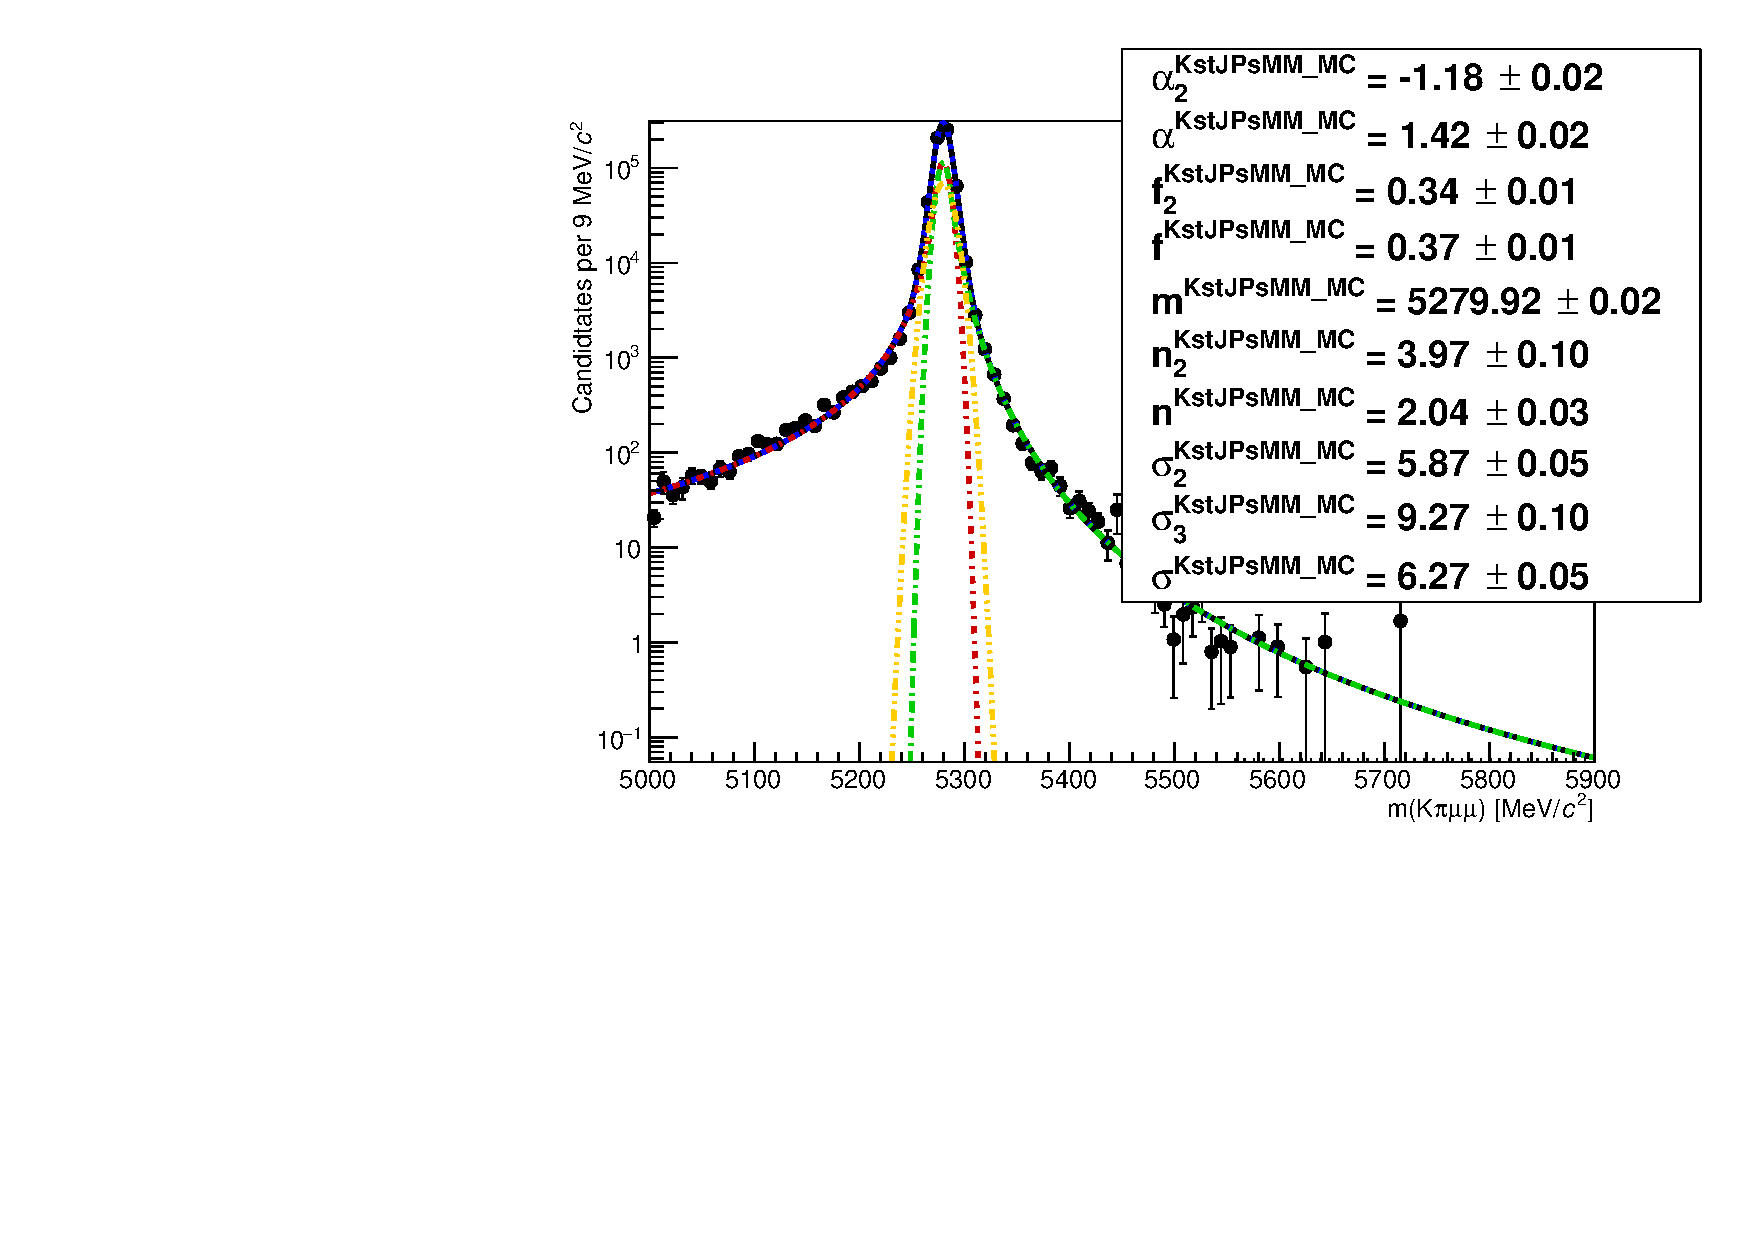
\includegraphics[width=0.7\textwidth]{RKst/figs/Fit/fit_MM/KstJPsMM_MC_log.pdf}
%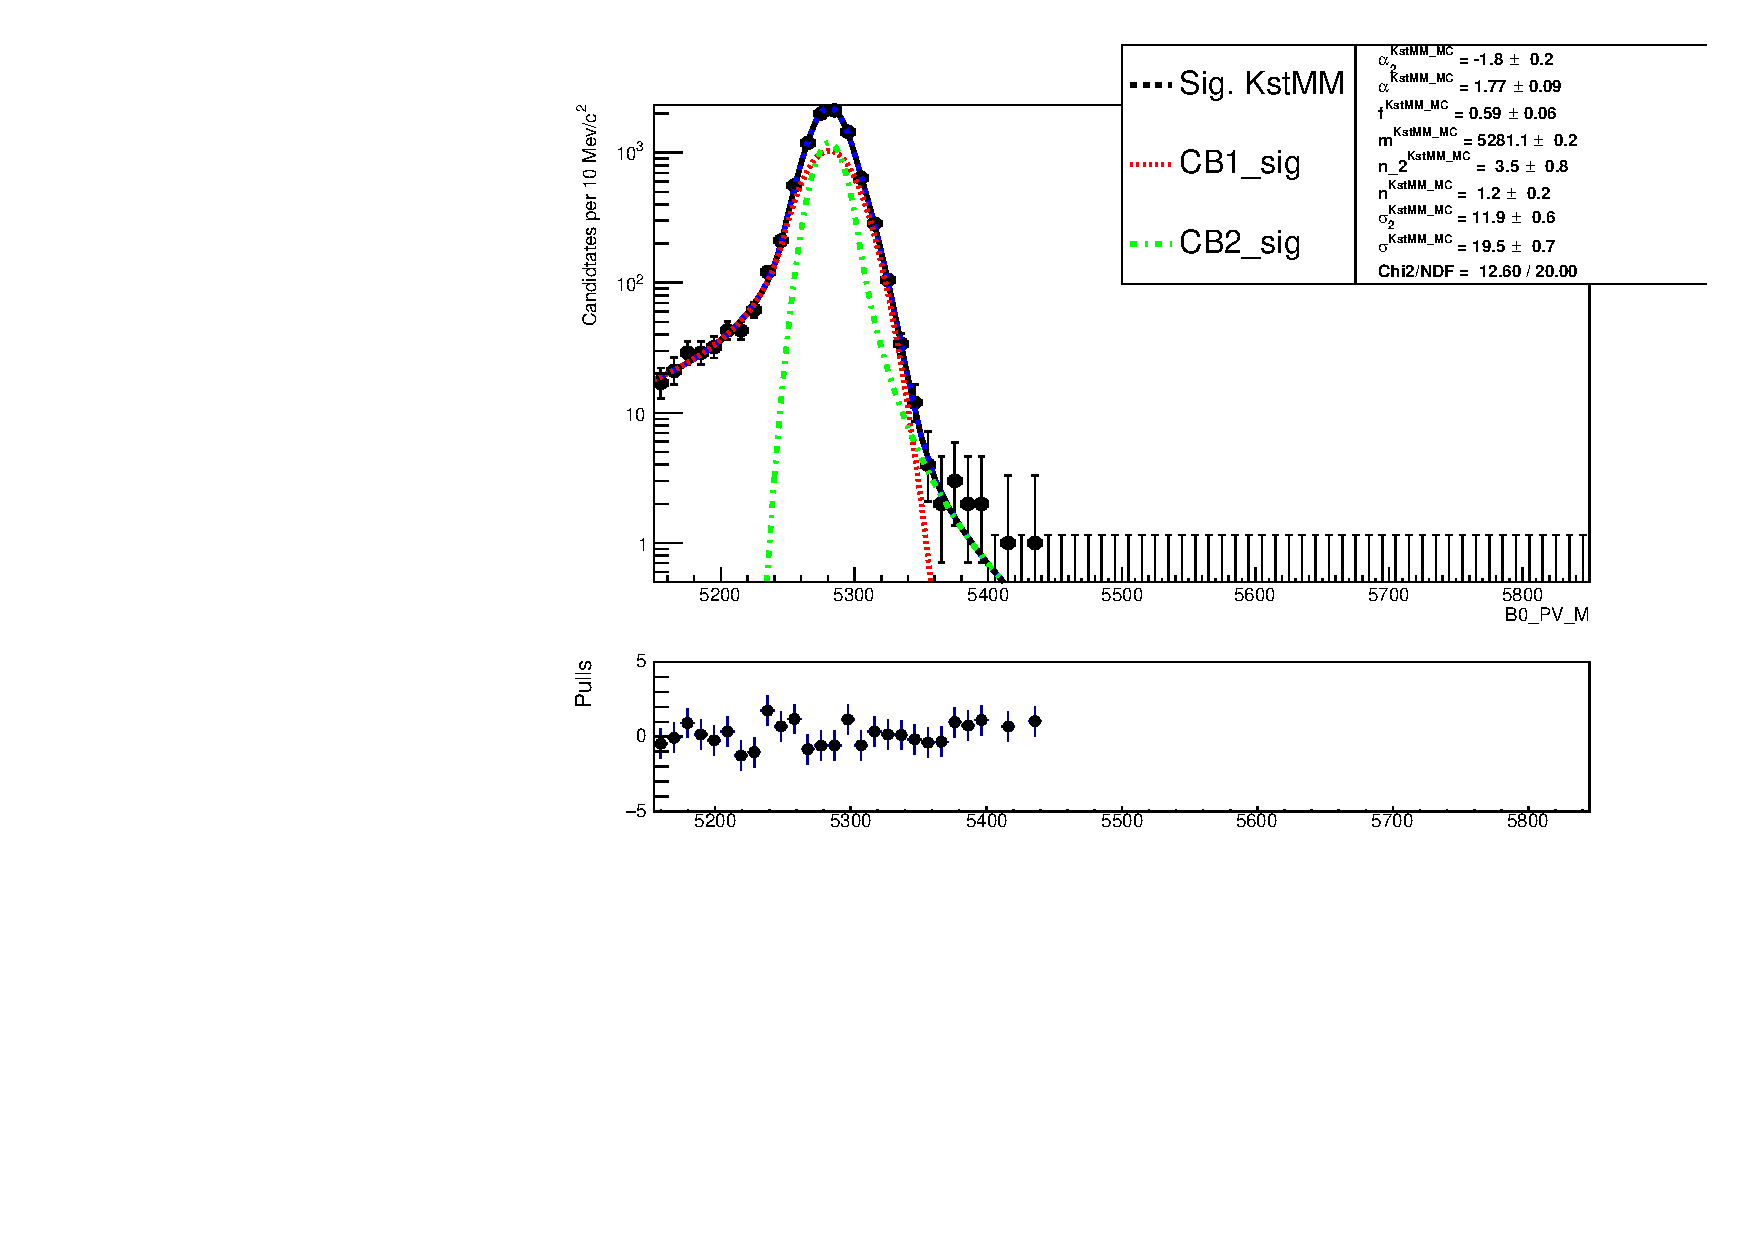
\includegraphics[width=0.48\textwidth]{figs/Fit/KstMM_MC_log_fitAndRes.pdf}
%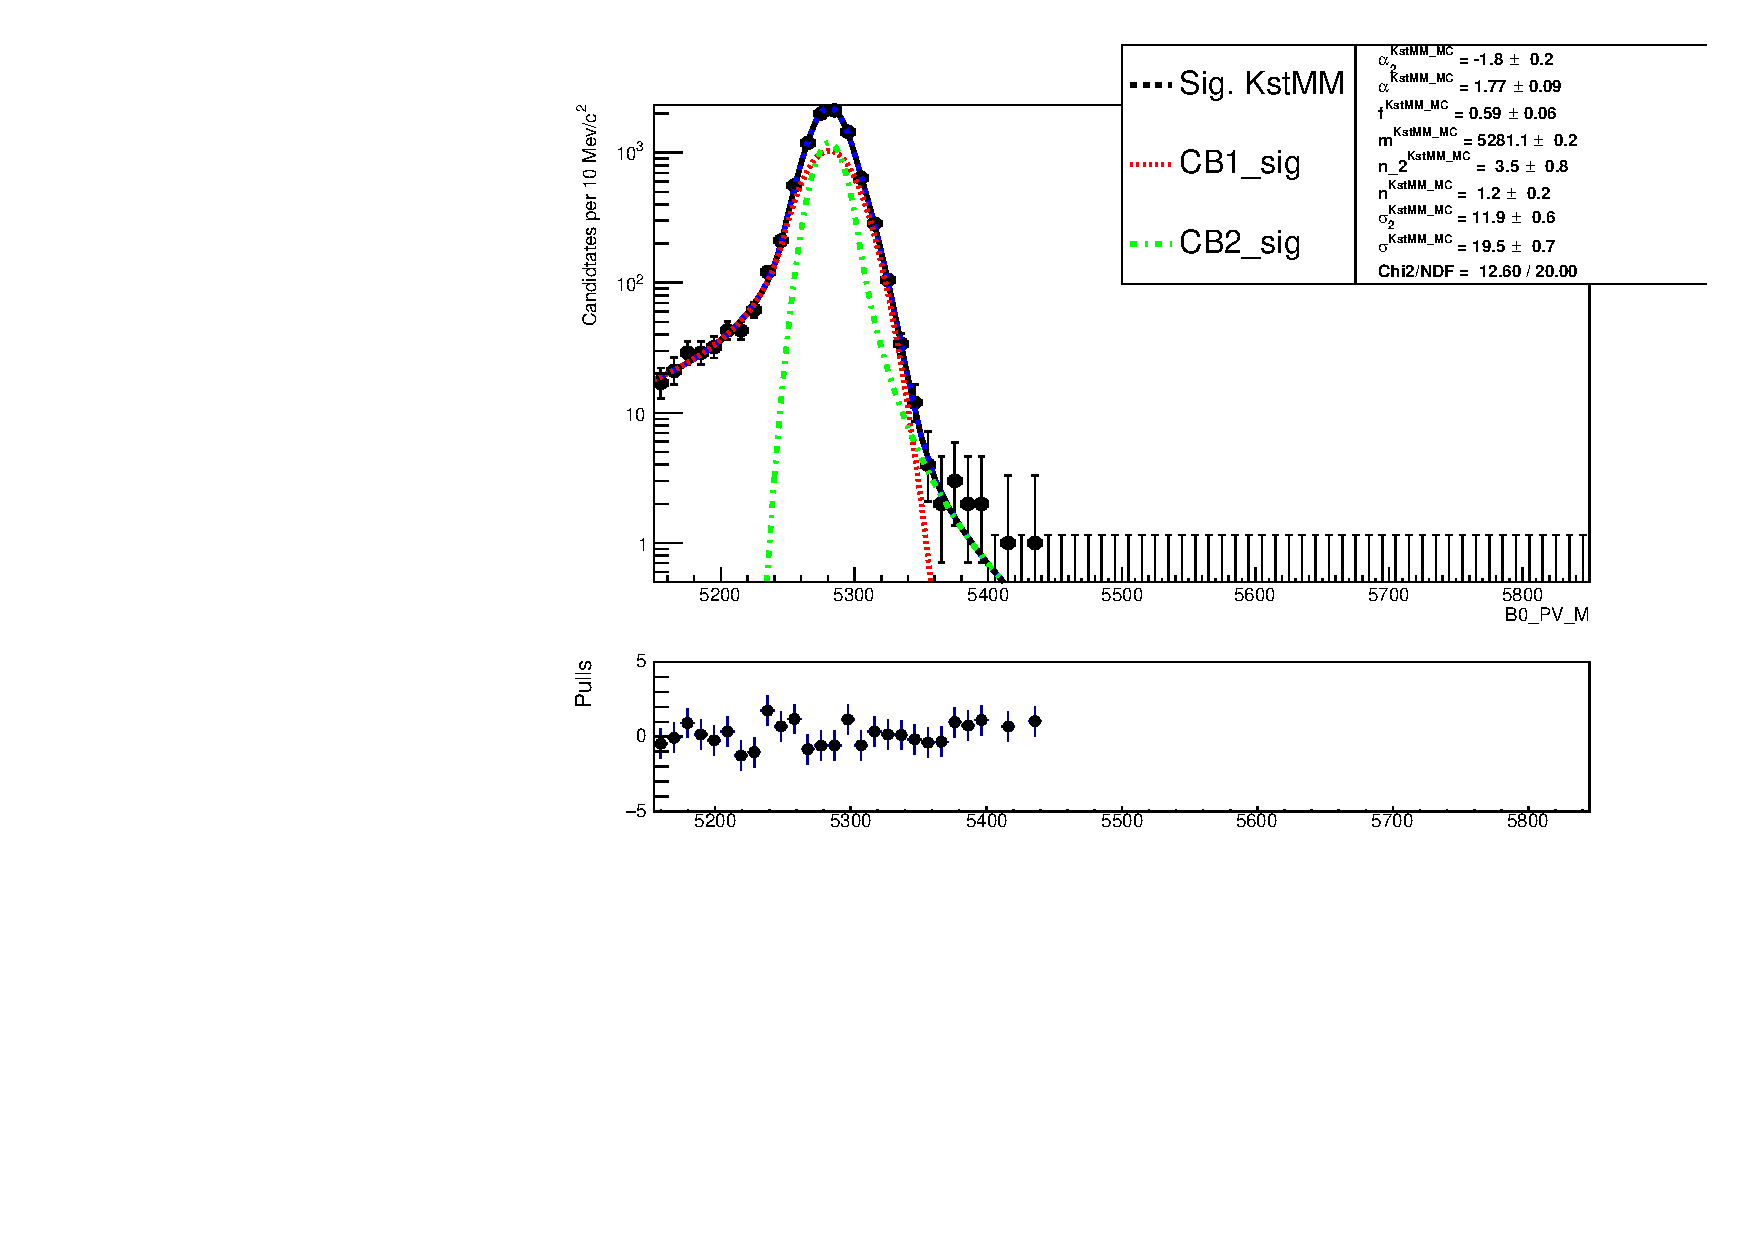
\includegraphics[width=0.48\textwidth]{figs/Fit/KstMM_MC_log_fitAndRes.pdf}
\caption{Fitted $m(K\pi \mu\mu)$ mass spectrum for $\Kstarz\jpsi$ simulated events. }
\label{fig:mumu_MC_fits}
\end{figure}

Then the fit to real data is performed. In order to do this the parameters of the signal PDF are fixed to the ones 
found fitting the simulated samples. However, in order to account for possible data-simulation discrepancies a scale
factor is multiplied to the widths and a shift is added to the masses and these are left free to vary. In summary the
PDFs used for the signal in the fits to data are defined as
%
\begin{equation}
\label{eq:DCB_RKst}
\begin{array} {ll}
DCB(m;c,m') = & f^{*} \cdot CB(m;\alpha_1^{*},n_1^{*},c \cdot \sigma_1^{*}, m_0^{*} + m') \\
&+ (1 - f^{*}) \cdot CB(m;\alpha_2^{*},n_2^{*},c \cdot \sigma_2^{*}, m_0^{*} + m')
\end{array}
\end{equation}  
%
where $f^{*}$ is the relative fraction of candidates falling in the first Crystal Ball function.
The free parameters are the width scale factor, $c$, and the mass shift, $m'$, which are common between
the rare and resonant samples. All the other parameters, denoted with $``^*"$, are taken from the fit to the
simulated candidates and are fixed when fitting data.

The background components considered for this fit are the following:
\begin{itemize}
\item (for rare and \jpsi) the combinatorial background modelled with an exponential function;
\item (only \jpsi) the $\Bs\to\Kstarz\jpsi$ background described using the same PDF used for the signal but a different
central value, $m_{0}$, which is set at the $\Bs$ nominal mass~\cite{PDG2014};
\item (only \jpsi) the $\Lb\to\jpsi pK$ background modelled using simulated \mbox{$\Lb\to\jpsi pK$} decays
to which the full selection is applied. The invariant mass distribution
of these candidates is a broad shape under the signal peak. The simulated distribution 
is smoothed using a kernel estimation method (using the \verb!RooKeysPdf! class of
the \textsc{RooFit} package~\cite{Verkerke:2003ir}).
\end{itemize}
%
\begin{figure}[h!]
\centering
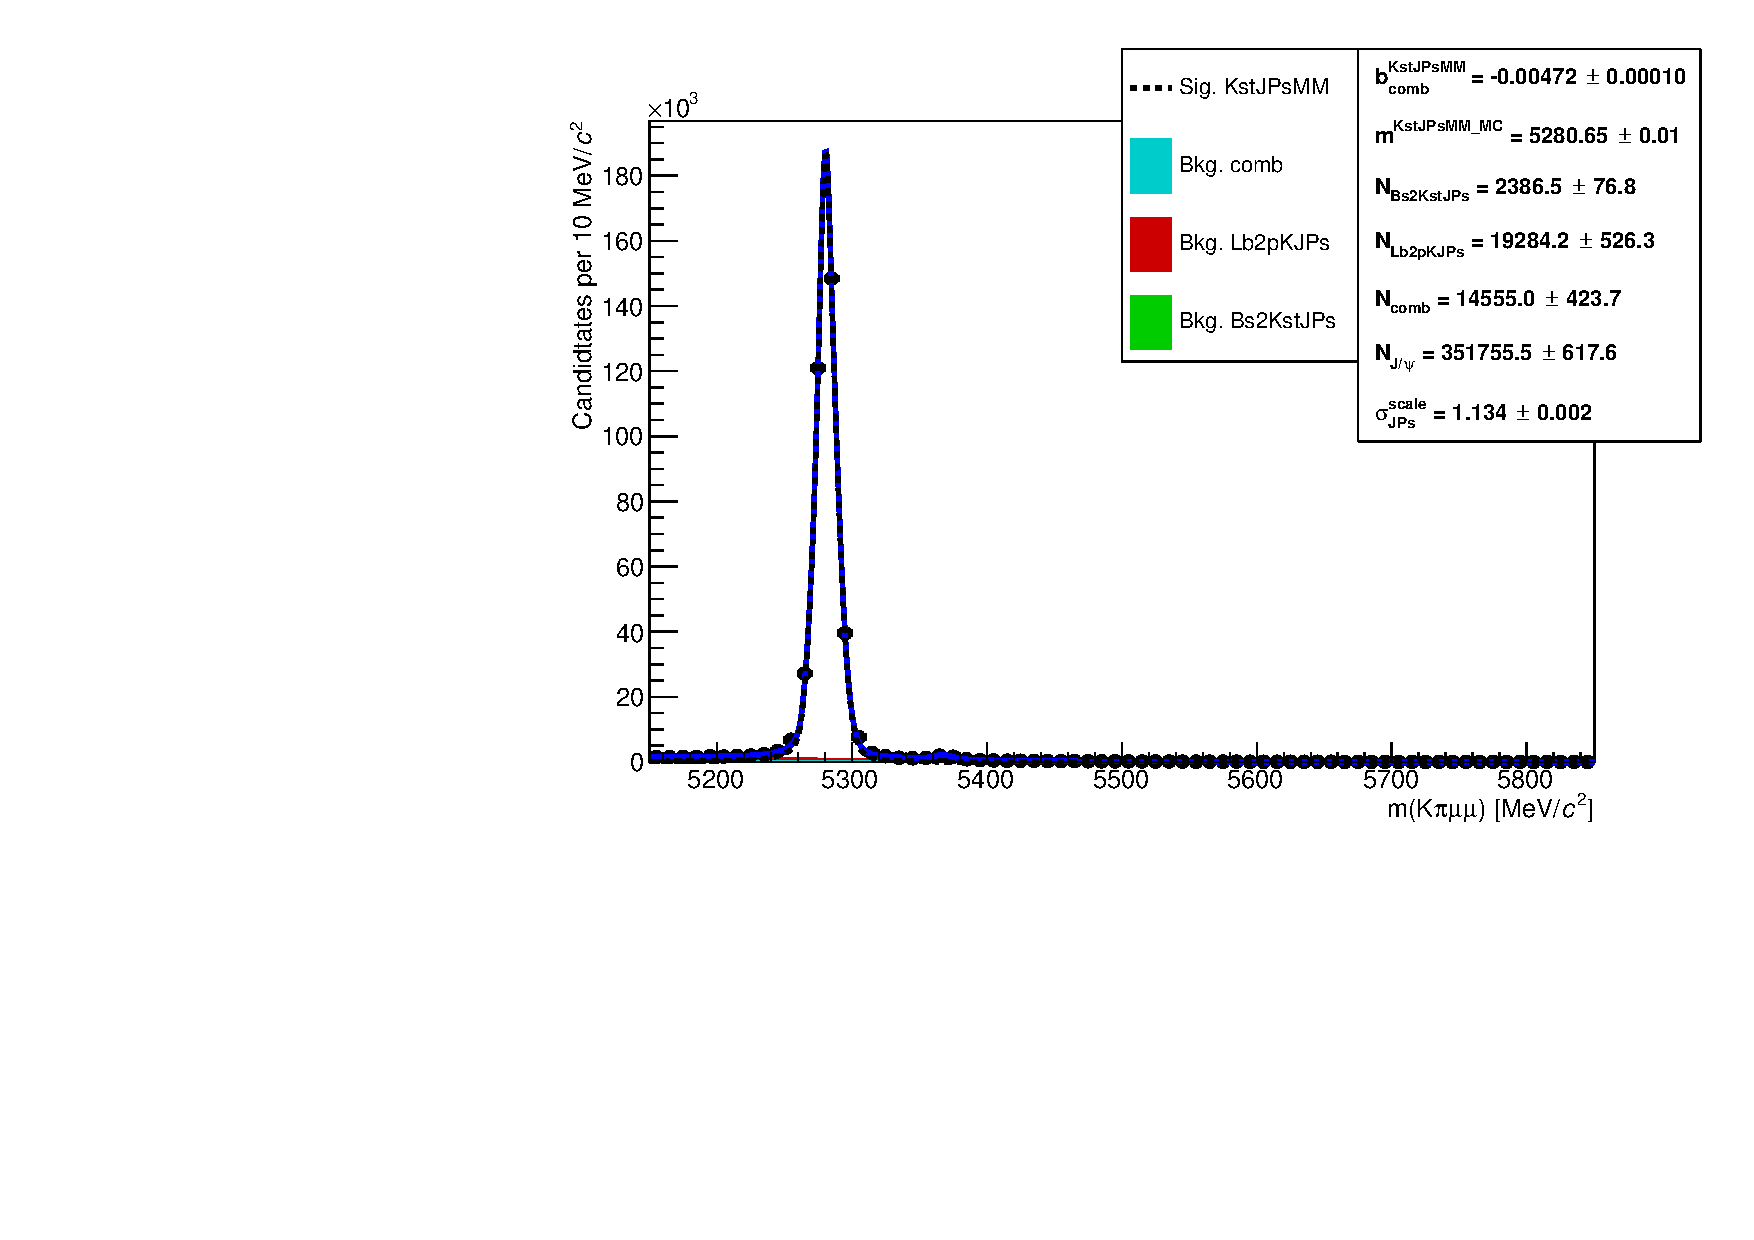
\includegraphics[width=0.49\textwidth]{RKst/figs/Fit/fit_MM/KstJPsMM.pdf}
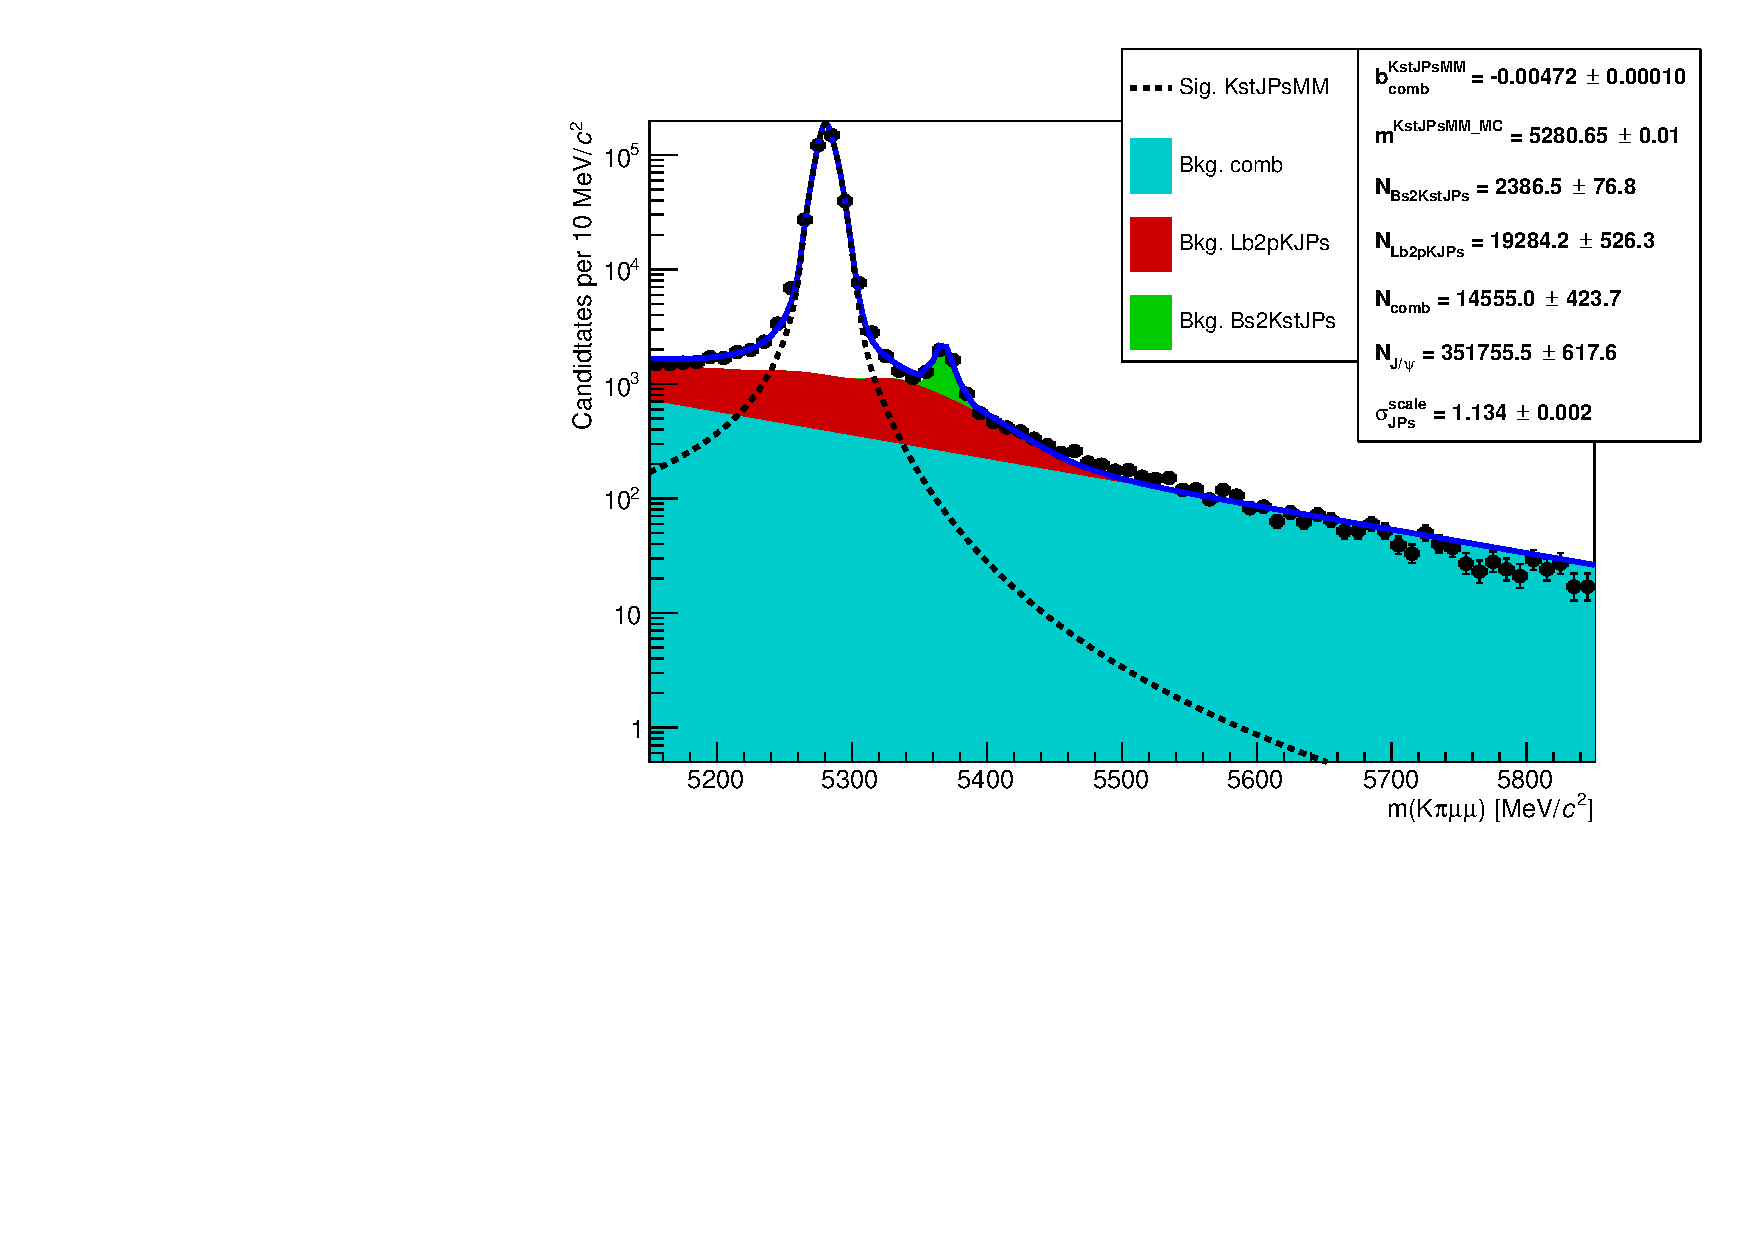
\includegraphics[width=0.49\textwidth]{RKst/figs/Fit/fit_MM/KstJPsMM_log.pdf}
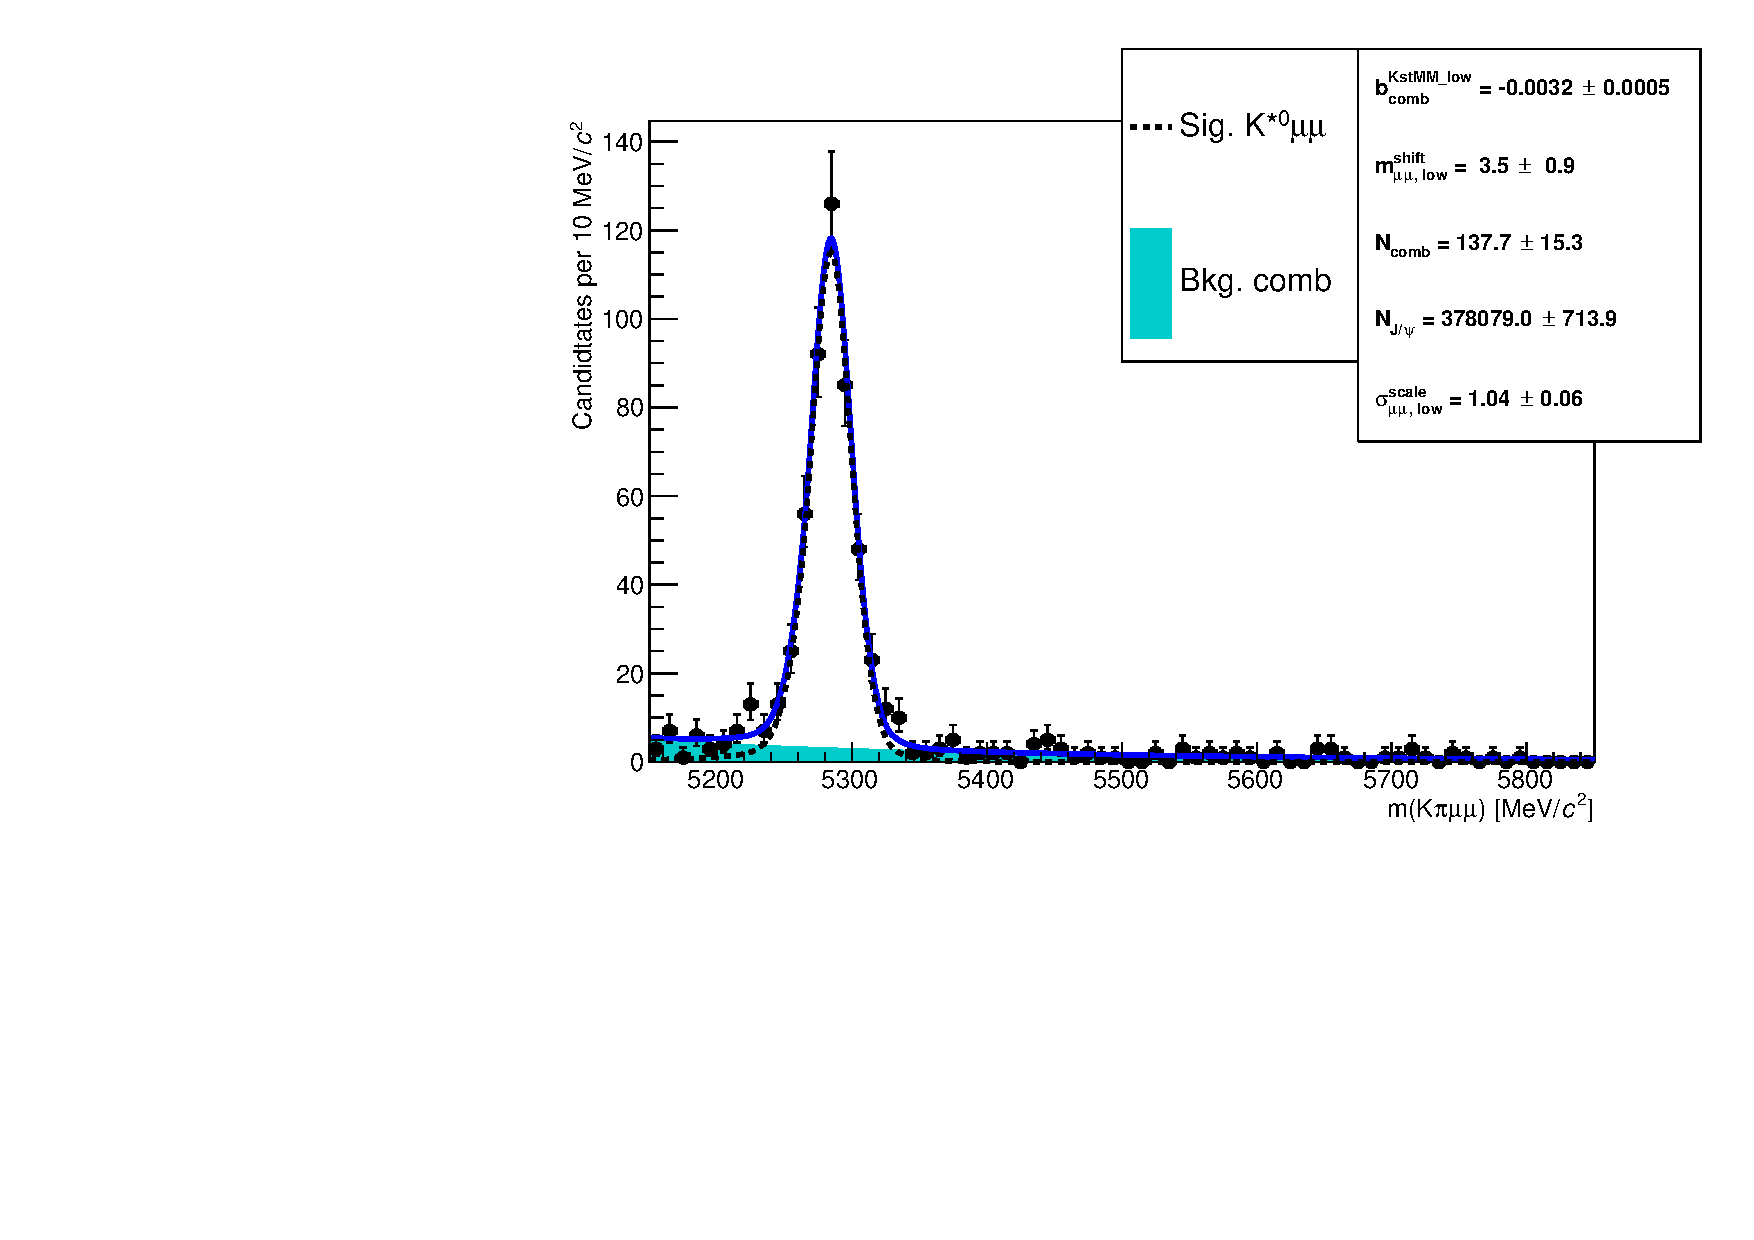
\includegraphics[width=0.55\textwidth]{RKst/figs/Fit/fit_MM/KstMM_low.pdf}
%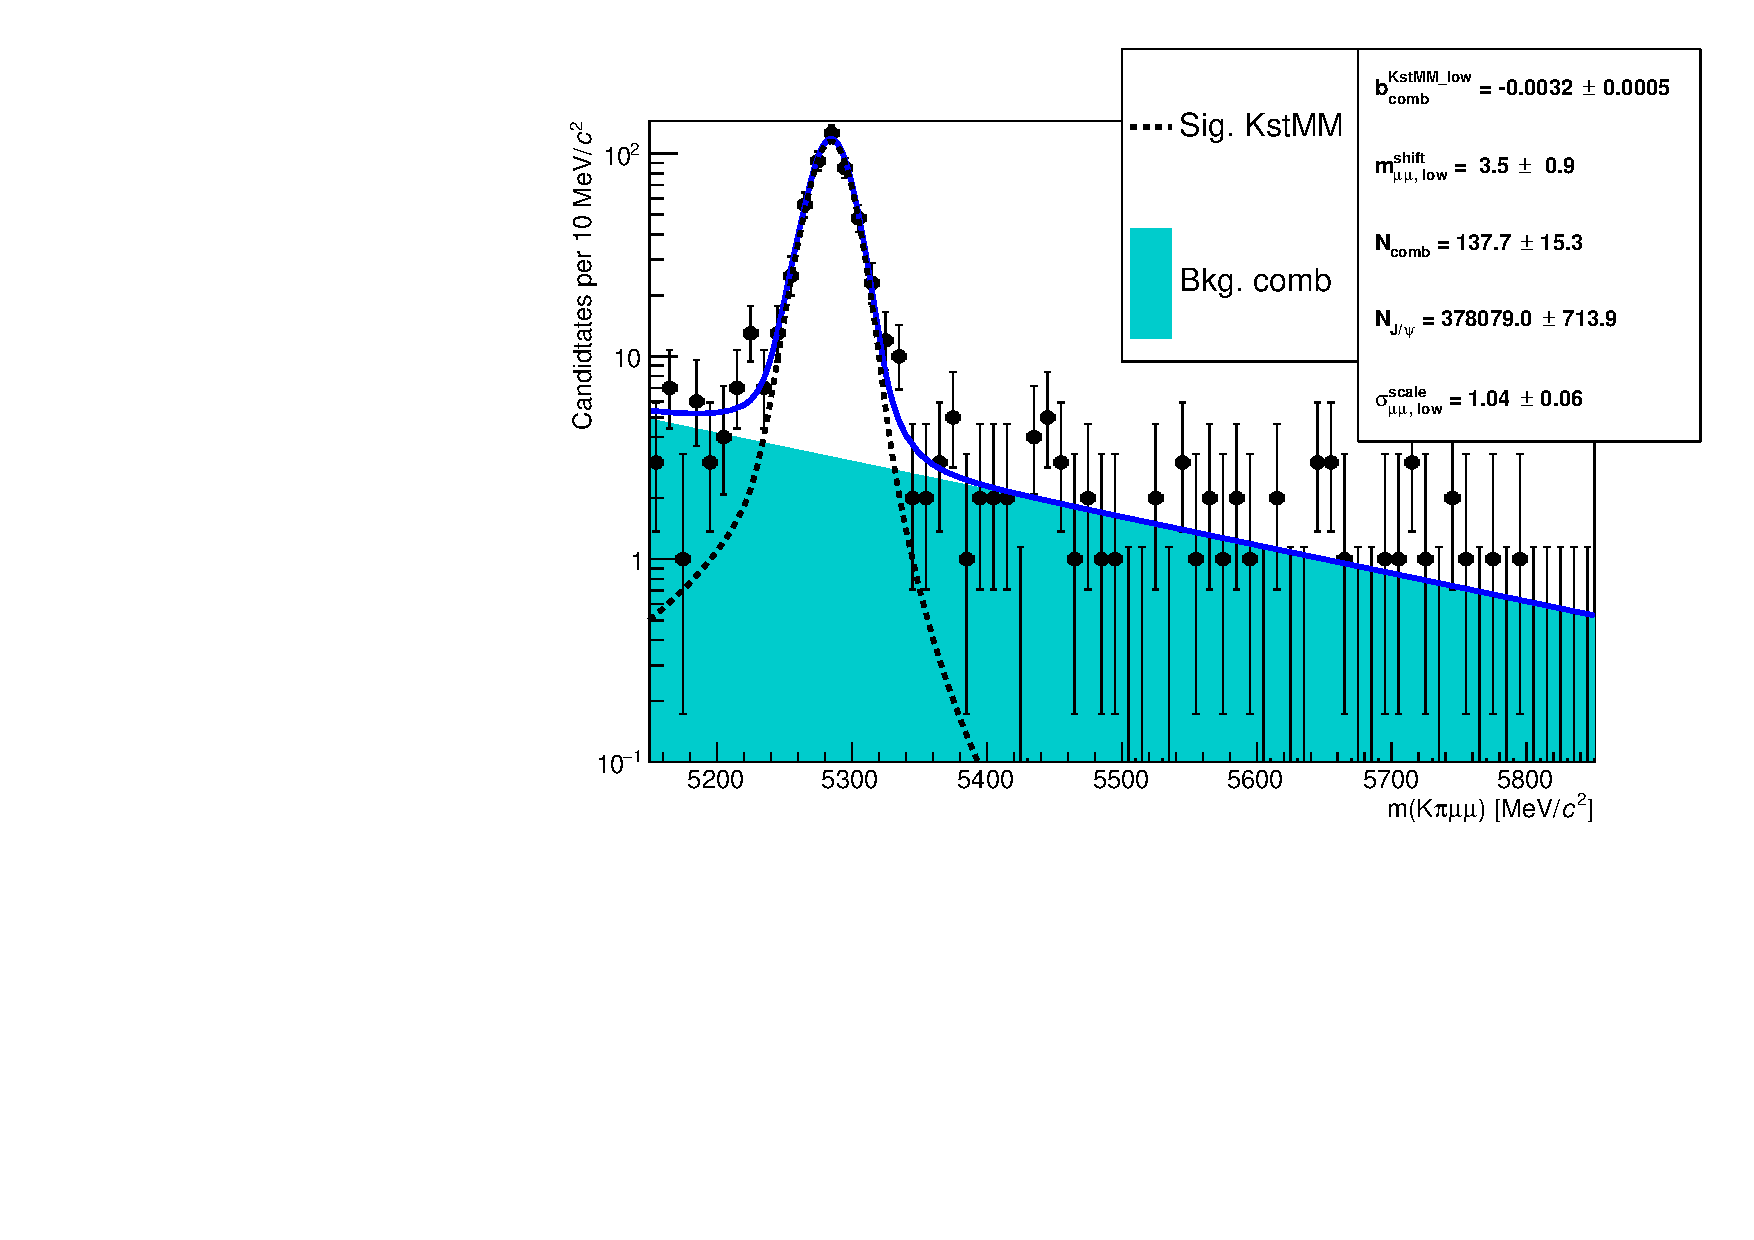
\includegraphics[width=0.49\textwidth]{RKst/figs/Fit/fit_MM/KstMM_low_log.pdf}
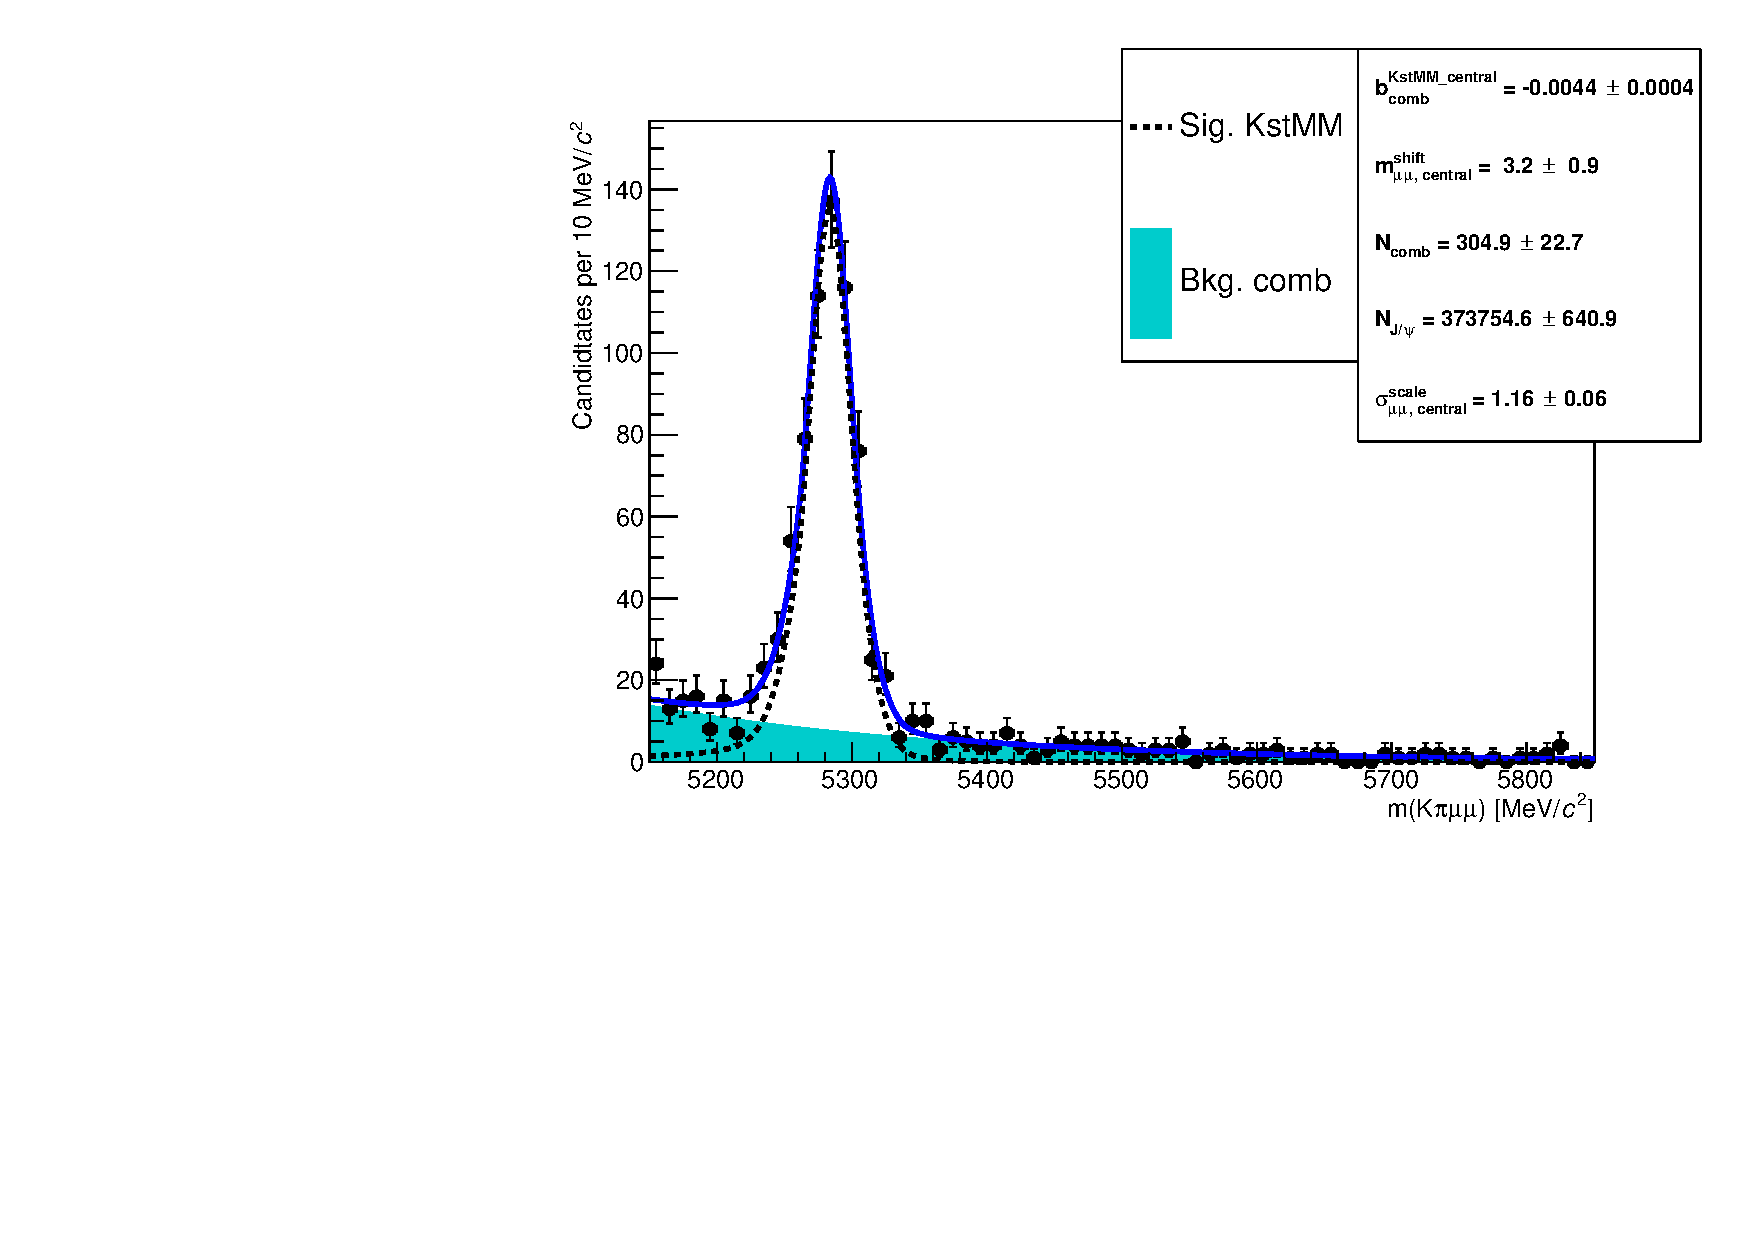
\includegraphics[width=0.55\textwidth]{RKst/figs/Fit/fit_MM/KstMM_central.pdf}
%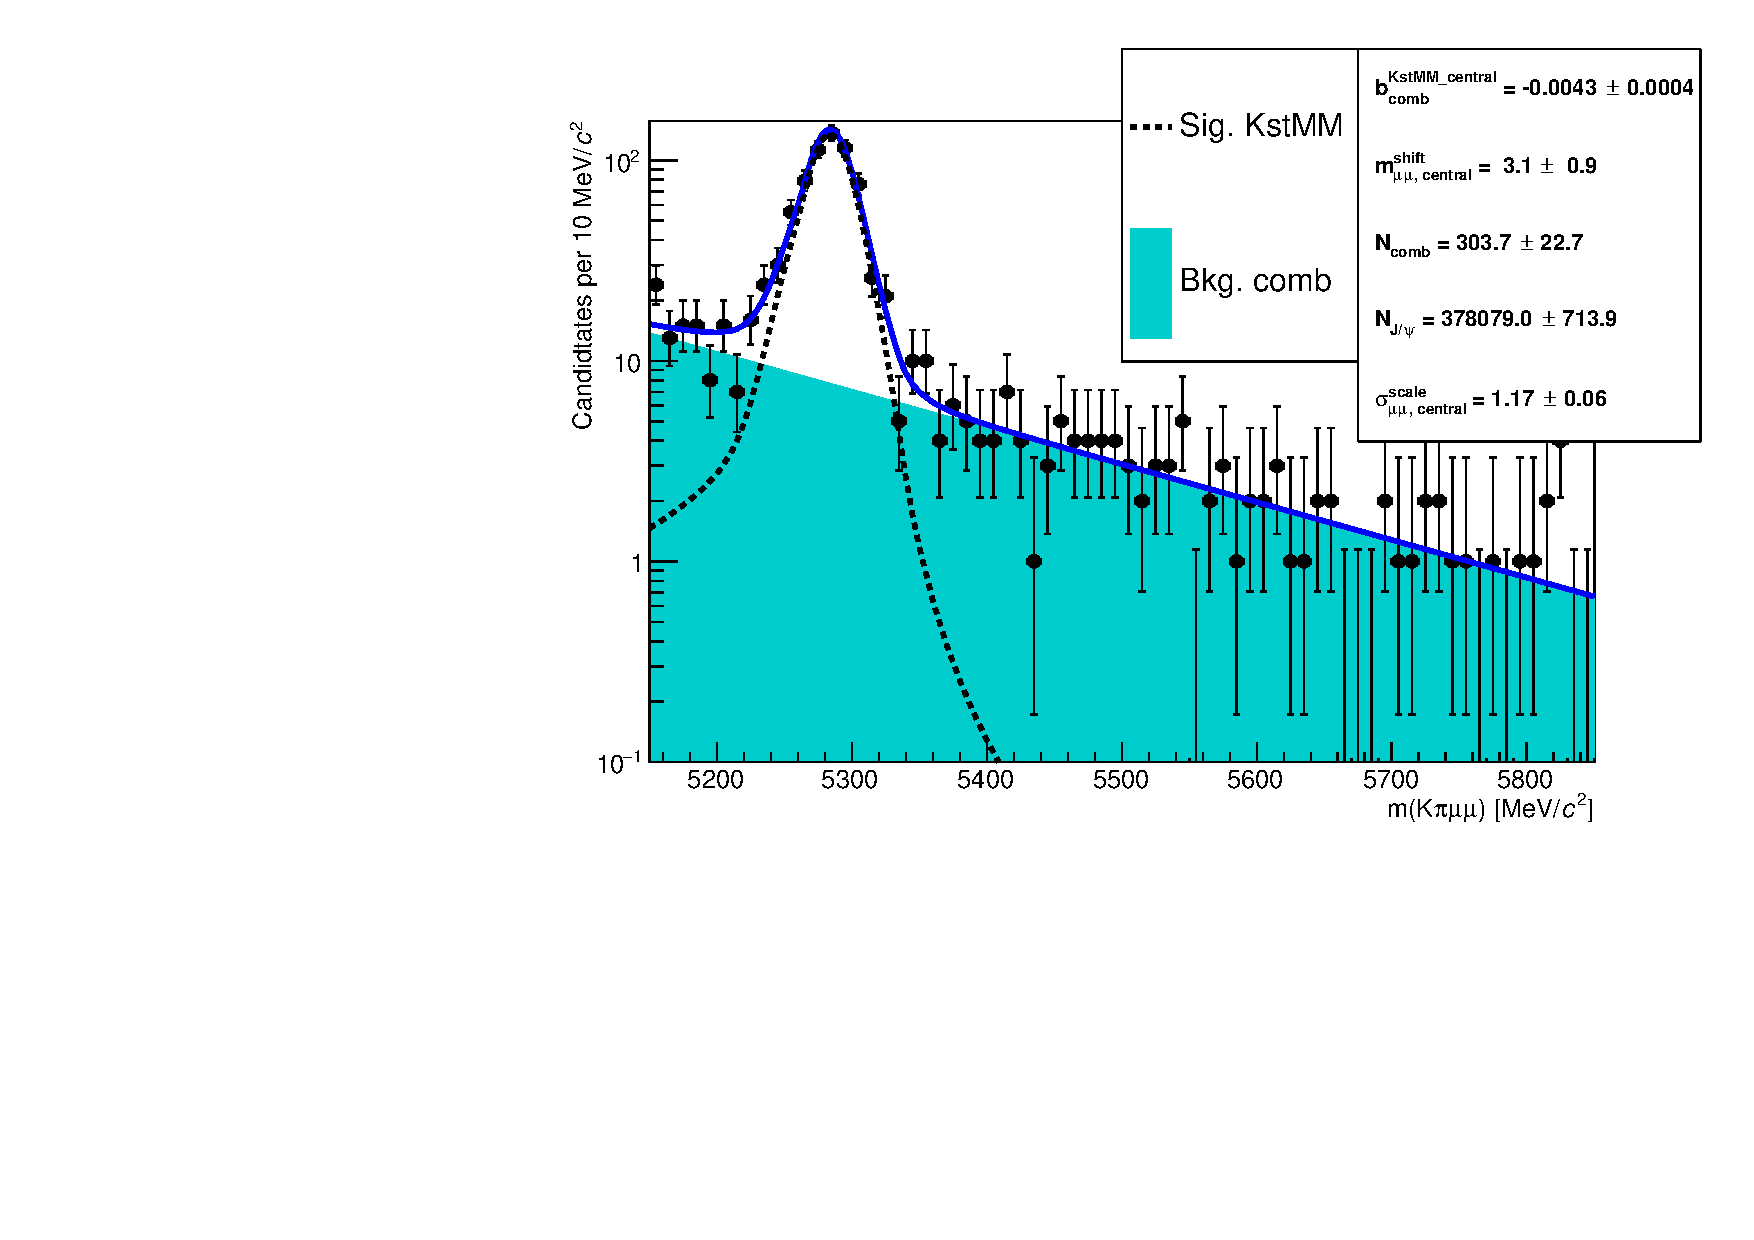
\includegraphics[width=0.49\textwidth]{RKst/figs/Fit/fit_MM/KstMM_central_log.pdf}
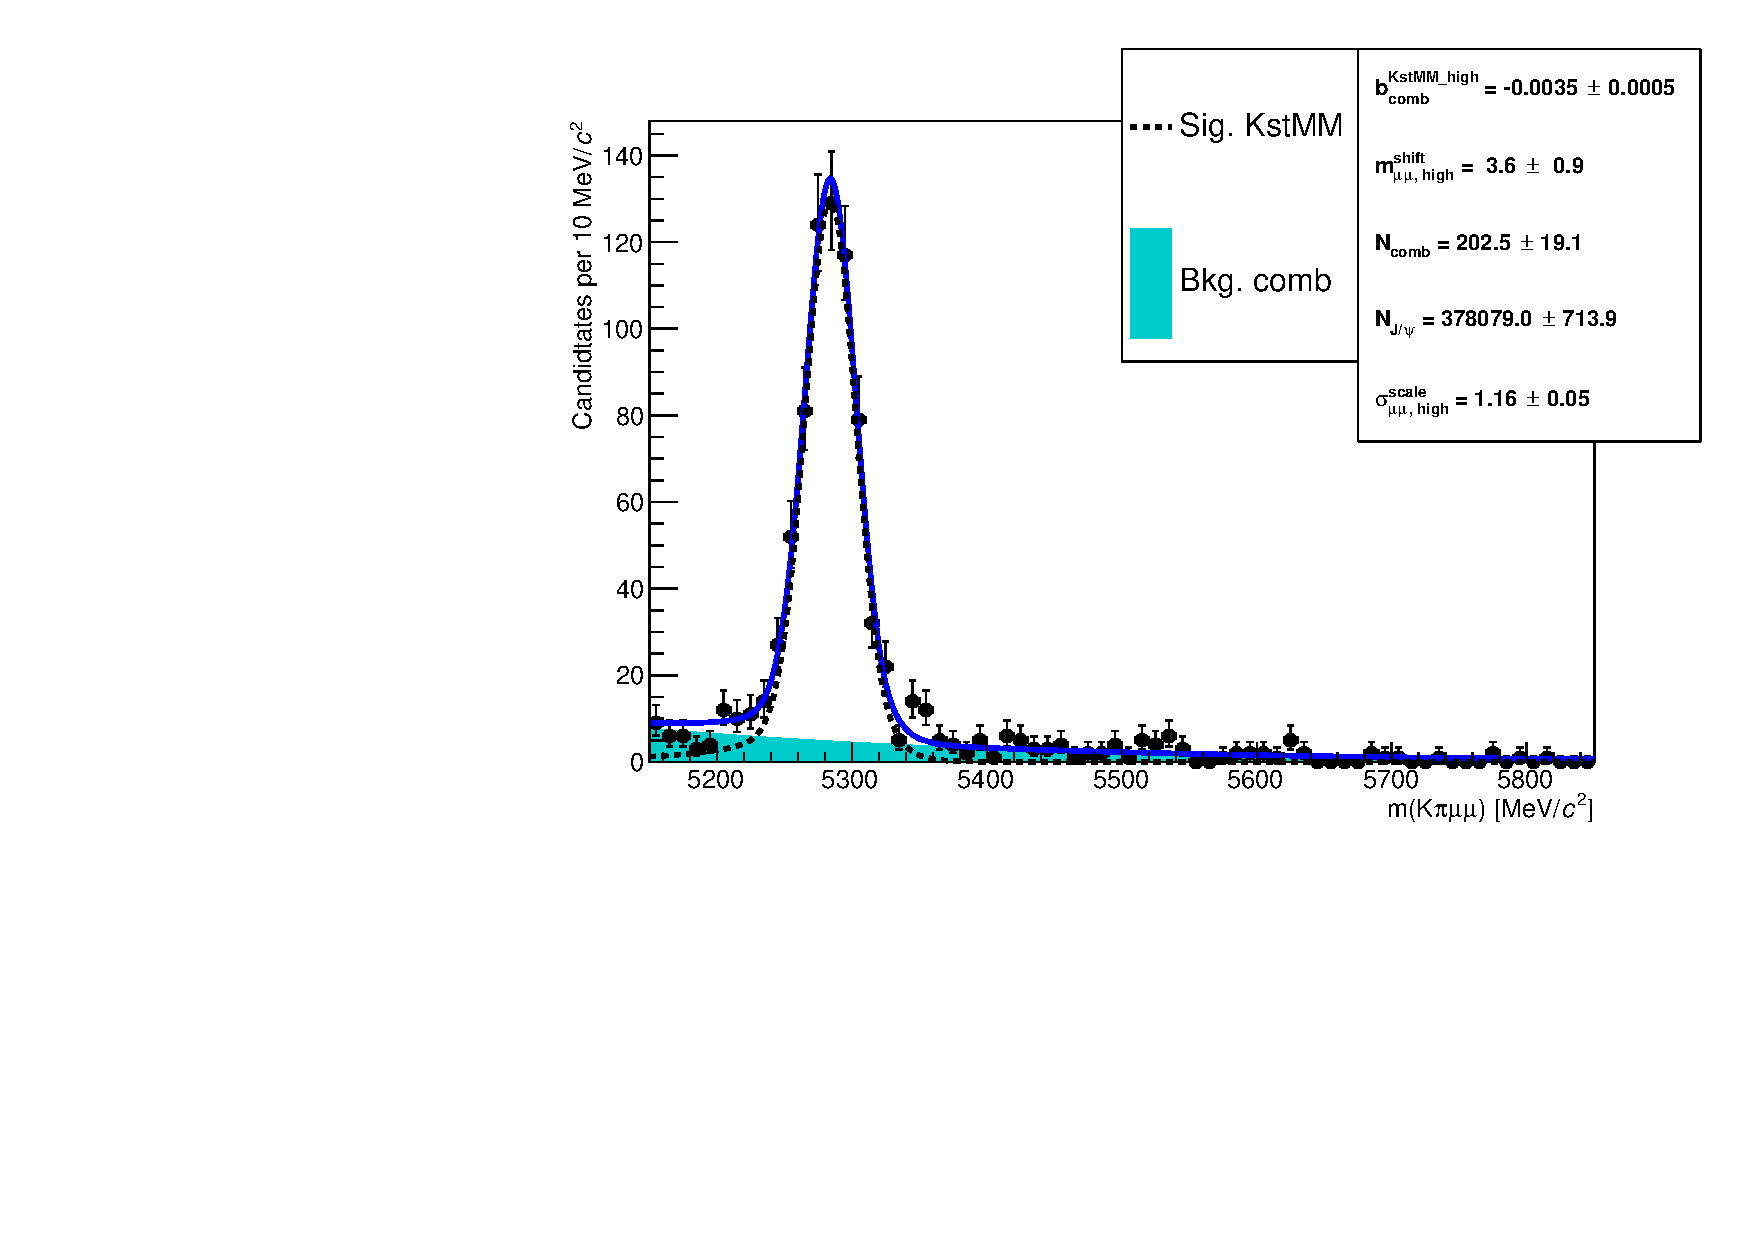
\includegraphics[width=0.55\textwidth]{RKst/figs/Fit/fit_MM/KstMM_high.pdf}
%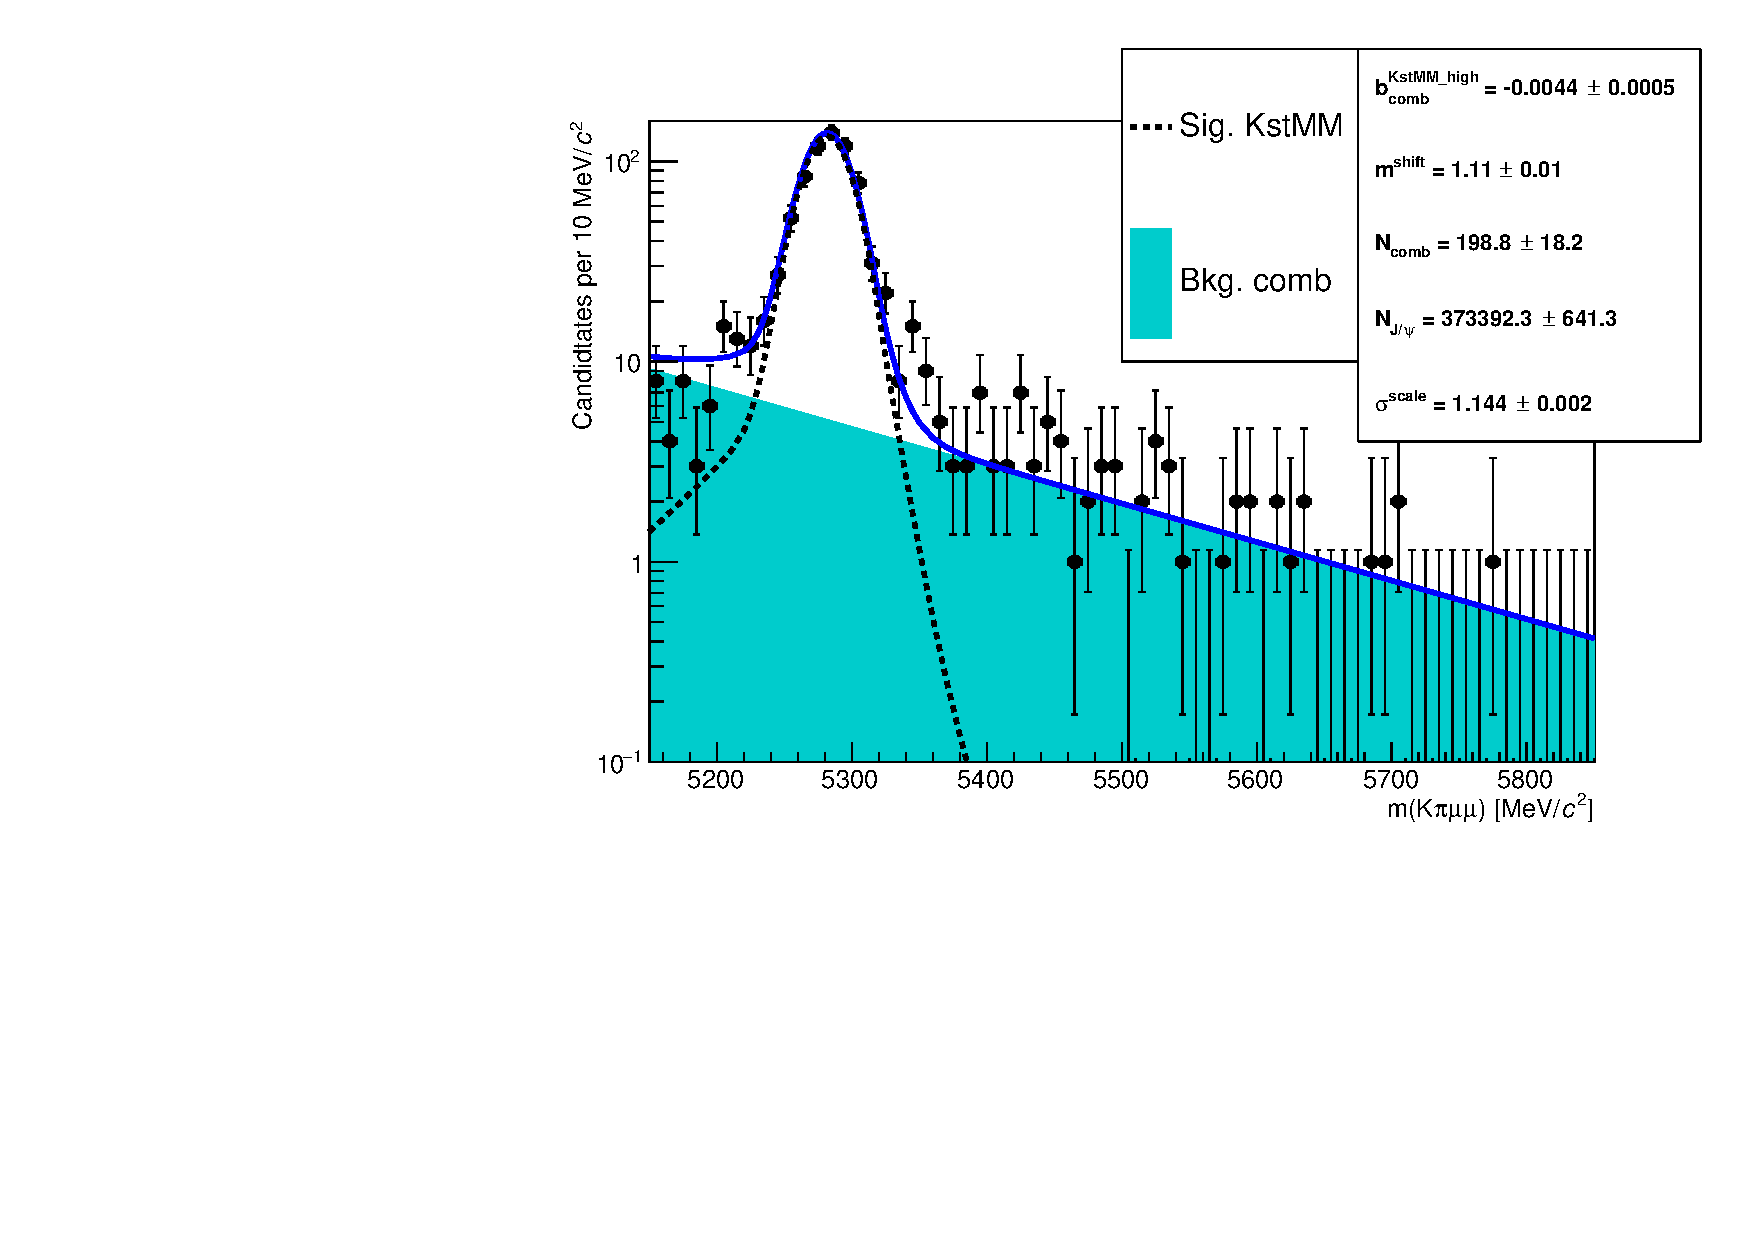
\includegraphics[width=0.49\textwidth]{RKst/figs/Fit/fit_MM/KstMM_high_log.pdf}
\caption{From top to bottom fitted $m(K\pi \mu\mu)$ invariant mass distributions
 for $\Kstarz\jpsi$ candidates and for rare candidates in the low-, central- and high-\qsq intervals.
Dashed black lines represent the signal PDFs and filled shapes the background components. }
\label{fig:mumu_data_fits}
\end{figure}

In summary the free parameters in the simultaneous fit to the $\mu\mu$ data samples are:
the signal and background yields, the combinatorial background slopes, and the data-MC
discrepancy parameters (the scale factor, $c$, and the mass shift, $m'$).
%
Figure~\ref{fig:mumu_data_fits} shows the results of the fit to the rare and resonant
$\mu\mu$ candidates. Values of the fitted parameters are reported on the plots.

\clearpage

\subsection{Electron channels}
\label{sec:RKst_fit_ee}

Also in the electron case the fit variable is the \mKpiee invariant mass coming from the kinematic
fit where all vertices are required to point to their mother particle. 
For the resonant samples a further constraint of the dilepton mass to the \jpsi and \psitwos nominal values is applied.
%
%In fact, due to the longer bremsstrahlung tail, the \jpsi mass constraint distorts the 4-body invariant mass
%distribution and makes it hard to model. Furthermore, mis-reconstructed background enters in the rare channel
%sample and its amount can be constrained by exploiting the higher statistics resonant channel, but this implies
%the usage of the same variable for both fits.
In order to better constrain the parameters modelling the radiative tail and the
backgrounds a wide mass window is used [4500,5800]~\mevcc. The lower limit is given
by the point in which the \qsq cut (at 6~\gevgevcccc to separate the rare and resonant channels)
starts to affect the 4-body invariant mass distribution. The control samples of \BdToKstPsiee and
\BdToKstGee candidates are also added to the simultaneous fit and a few parameters are shared as explained later.
Finally, for the \BdToKstJPsee candidates the invariant mass calculated without \jpsi mass constraint
is also added to the fit as a control sample. This is necessary in order to obtain the data-simulation discrepancy parameters
shared with the model for the rare samples, which requires to fit the same variable in both cases.

The invariant mass distributions are different depending on the
trigger category and the number of bremsstrahlung photons recovered.
%Furthermore the efficiencies can be more easily treated if divided in trigger categories.
Therefore, our samples are divided in three trigger categories, as described in
Sec.~\ref{sec:RKst_trigstripping}, and three bremsstrahlung categories defined as:
%
\begin{itemize}
\item $0\gamma$: candidates with no photon emitted
\item $1\gamma$: candidates with one photon by either of the electrons
\item $2\gamma$: candidates with ono photon emitted by each electron
\end{itemize}
%
The three samples, divided by trigger, are fitted simultaneously.
This allows a better use of the available statistics as the simultaneous fit
gathers information from the three categories at the same time.
Furthermore, using this method the results for the three categories are
naturally combined in a single $r_{ee}$ ratio.
%
The PDFs used to fit the invariant mass distributions are described in the next subsections.



\subsubsection{Signal PDFs for the electron channels}
\label{sec:fit_ee_central}


\begin{table}
\centering
\caption{Percentages of events with 0, 1 and 2 emitted photons in the three
trigger categories, obtained from simulated events.}
\begin{tabular}{|c|ccc|}
\hline
Trigger 	&	$0 \gamma$ (\%)	&	$1 \gamma$   (\%) &	 $2 \gamma$ (\%) \\ \hline
\multicolumn{4}{|c|}{\BdToKstee low-\qsq} \\ \hline
L0E			&	34.2	&	56.0		&	9.8	 \\
L0H			&	27.8	&	58.1		&	14.2	 \\
L0I			&	31.7 	&	56.9		&	11.4	 \\
\hline
\multicolumn{4}{|c|}{\BdToKstee central-\qsq} \\ \hline
L0E			&	29.2 	& 50.0 		& 20.8	 \\
L0H			&	23.6 	& 50.5 		& 26.0	 \\
L0I			&	28.5 	& 49.9 		& 21.6	 \\
\hline
\multicolumn{4}{|c|}{\BdToKstee high-\qsq} \\ \hline
L0E			&	20.6 	& 51.2 		& 28.2	 \\
L0I			&	10.0 	& 53.8 		& 36.2 \\
\hline
\multicolumn{4}{|c|}{\BdToKstGee} \\ \hline
L0E			&	40.4	&	59.6	&	--	 \\
L0H			&	32.2	&	67.8	&	--	 \\
L0I			&	39.3 	&	60.7	&	--	 \\
\hline
\multicolumn{4}{|c|}{\BdToKstJPsee} \\ \hline
%\multicolumn{4}{c}{\small (vertex constrained)} \\ \hline
%L0E			&	28.947 & 50.100 & 20.952	 \\
%L0H			&	18.873 & 51.128 & 29.999	 \\
%L0I			&	26.724 & 51.698 & 21.578	 \\
%\hline
%\multicolumn{4}{c}{\small (vertex and mass constrained)} \\ \hline
L0E			&	29.0 	& 50.1 		& 20.8	 \\
L0H			&	18.9 	& 51.3 		& 29.8	 \\
L0I			&	26.9 	& 51.7 		& 21.4	 \\
\hline
\multicolumn{4}{|c|}{\BdToKstPsiee} \\ \hline
L0E			&	27.2 & 51.3 & 21.5	 \\
L0H			&	17.4 & 51.5 & 31.2	 \\
L0I			&	22.0 & 55.0 & 23.0	 \\
\hline
\end{tabular}
\label{tab:brem_frac}
\end{table}

As for the muonic channel, simulated events are fitted fist to constrain
the shape parameters for the subsequent fit to data. The signal PDFs are built using the following method:
%
\begin{itemize}
\item Simulated $\Bz\to\Kstarz\jpsi(ee)$ and $\Bz\to\Kstarz ee$ events are divided
in each trigger and bremsstrahlung category and an independent fit is performed to each sample.
A different fit is also performed for the central, \jpsi and high \qsq intervals. In the case of the high-\qsq 
interval it is particularly important to keep signal tail parameters independent from \jpsi channel ones
because, as can be seen in Fig.~\ref{fig:high_central_mass_comparison}, the invariant mass
distributions are significantly different for the two intervals.
\item For each trigger category a PDF is built as the sum of the three PDFs of the bremsstrahlung categories:
\begin{equation}
P(m)^{\rm trg} = f^{\rm trg}_{0\gamma} P^{\rm trg}_{0\gamma}(m) + f^{\rm trg}_{1\gamma} P^{\rm trg}_{1\gamma}(m) + (1 - f^{\rm trg}_{0\gamma} - f^{\rm trg}_{1\gamma}) P^{\rm trg}_{2\gamma}(m),
\end{equation}
where the $P(m)^{trg}_{n\gamma}$ functions are the chosen PDFs for the trigger and bremsstrahlung categories
and the $f^{trg}_{n\gamma}$ parameters are the relative fractions of events falling in each category.
\item Most parameters are fixed (details later) and the combined PDF, $P(m)$,
is used to fit real data divided only in trigger categories.
\end{itemize}
%
\begin{figure}[h!]
\centering
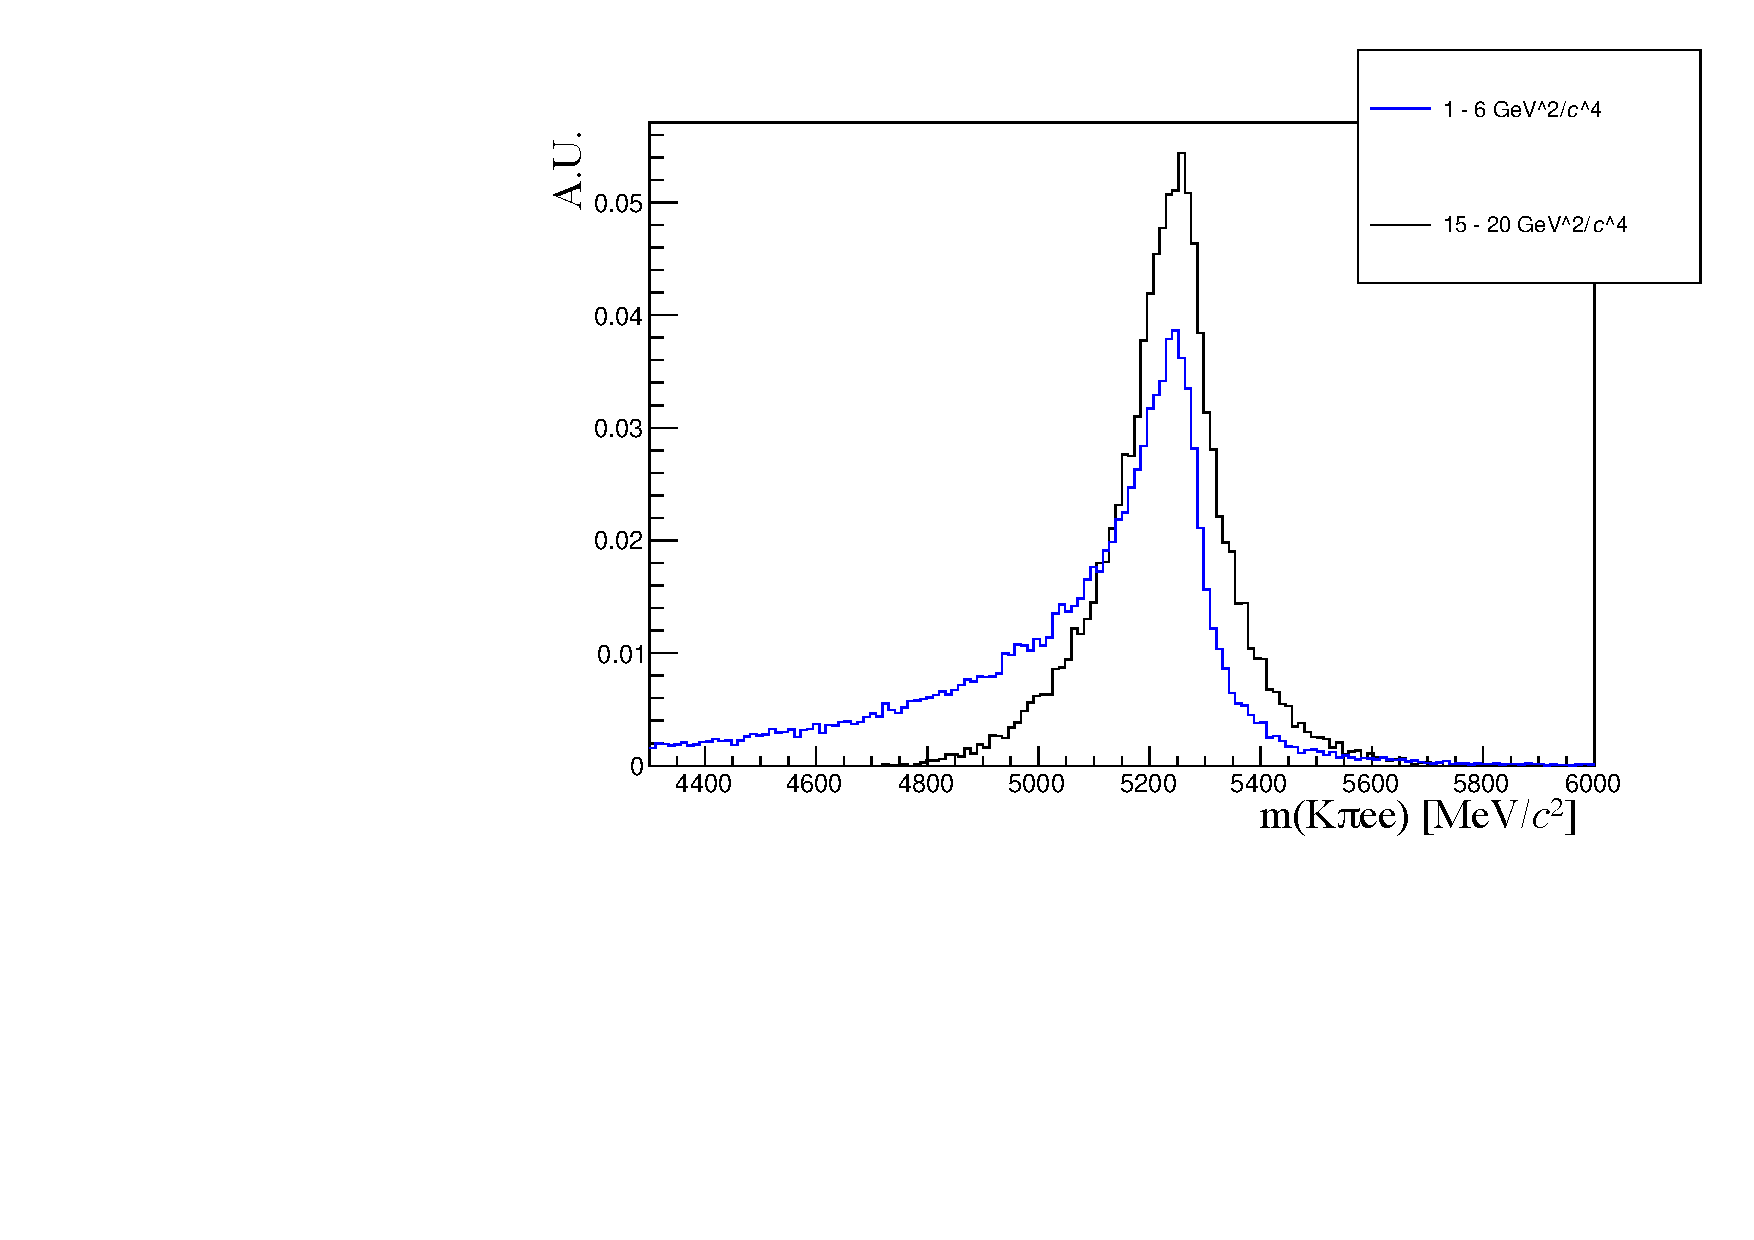
\includegraphics[width=0.70\textwidth]{RKst/figs/high_central_mass_comparison.pdf}
\caption{Simulated invariant mass of the $K\pi ee$ system in the $1.1 < \qsq < 6$ and $\qsq > 15$~\gevgevcccc intervals.  }
\label{fig:high_central_mass_comparison}
\end{figure}

The $0\gamma$ category is characterised by a better resolution and a sharp tail on the righthand
side and it is fitted with a simple Crystal Ball function (CB). Instead the $1\gamma$ and $2\gamma$
samples are modelled using the sum of a Crystal Ball and a Gaussian functions (CBG) with all parameters independent.
When the combined PDF, $P(m)^{\rm trg}$, is built all parameters are fixed leaving one global mass shift 
and one scale factor for the widths free to vary, as done for the muonic samples.

%Finally, combining the three bremsstrahlung PDFs one needs to specify in which fractions they contribute to the total.

The $f^{trg}_{n\gamma}$ fractions have been shown to be in good agreement between 
resonant data and simulation and therefore they are fixed to the simulated values, separately
for the normalisation channel and each \qsq interval. Table~\ref{tab:brem_frac} lists the percentages
of candidates with 0, 1 and 2 recovered photons for each trigger category.

In summary the signal PDF for the fit on data is defined as:
%
\begin{equation}
\begin{array} {ll}
P(m;c,m')^{\rm trg} & = f^{\rm trg}_{0\gamma} \text{CB}^{\rm trg}_{0\gamma}(m;c,m')  \\
& + f^{\rm trg}_{1\gamma} \text{CBG}^{\rm trg}_{1\gamma}(m;c,m') + (1 - f^{\rm trg}_{0\gamma} - f^{\rm trg}_{1\gamma}) \text{CBG}^{\rm trg}_{2\gamma}(m;c,m')
\end{array} 
\end{equation}
%
where the free parameters are: $c$, the scaling factor for the widths, and $m'$, the mass shift.


\subsubsection{Background PDFs for the electron channels}
\label{sec:RKst_misreco_fit}

This section reports the background components considered for the fit to each sample.

\subsubsection*{\BdToKstGee}

\begin{itemize}

\item \textit{Combinatorial}: described using an exponential function; the yield and slope parameters are free to vary in the fit;

\item \textit{Partially-reconstructed} (hadronic): the shape is obtained from simulation similarly to the $\jpsi(ee)$ mode. 
However, as there are no inclusive samples for the rare channel, a sample including higher \Kstarz resonances, 
such as $K_1^+(1270)$, which is the dominant component, is used.; the yield is left free to vary.

\end{itemize}


\subsubsection*{\BdToKstJPsee and \BdToKstPsiee}

The following backgrounds are considered for the fits to the vertex constrained invariant mass 
of \BdToKstJPsee candidates:
%
\begin{itemize}

\item \textit{Combinatorial}: described using an exponential function. The yield and slope parameters are free to vary in the fit;

\item \textit{Partially-reconstructed}: this background is split in an hadronic component, involving higher hadronic resonances, and a leptonic one, coming from higher \ccbar resonances. Both categories are modelled using inclusive \decay{\Bz}{\jpsi X} simulated events to which the full selection is applied. The distribution for the hadronic (leptonic) category is defined by selecting candidates where the \Kstarz (\jpsi) is not a direct daughter of the \Bz. The invariant mass distributions of these candidates, shown in Fig.~\ref{fig:misreco}, are smoothed using a kernel estimation method and their yields are left free to vary in the fit. Given the little statistics available, the same shape is used for all the trigger categories;

\item $\Bz\to\Kstarz(\psitwos\to\ee)$: the leakage from the \psitwos radiative tail into the \jpsi interval is modelled by selecting simulated $\psitwos\to\ee$ events falling into the \jpsi mass window (6--11\gevgevcccc). The normalisation is fixed to the $\Bd\to\Kstarz(\psitwos\to\ee)$ yield, $N_{\psitwos(ee)}$, as:
%
$$N_{\jpsi(ee)}^{\rm leak} = N_{\psitwos(ee)} \cdot f_{\psitwos(ee)}^{\rm leak, \,MC},$$
%\frac{N_{\psitwos(ee)}^{\rm leak, \,MC}}{N_{\psitwos(ee)}^{\rm MC}},$$
%
where $f_{\psitwos(ee)}^{\rm leak, \,MC}$ is the fraction of $\Bd\to\Kstarz(\psitwos\to\ee)$ simulated events reconstructed in the \jpsi interval.

\item $\Lb\to pK(\jpsi\to\ee)$: described using simulated events to which the full selection is applied. This distribution has a broad shape under the signal peak and is smoothed using a \texttt{RooKeysPdf}. The normalisation is constrained to the $\Lb\to pK(\jpsi\to\mumu)$ yield returned by the $\mu\mu$ fit after correcting for efficiency differences between final states with muons and electrons.

\item $\Bs\to\Kstarz(\jpsi\to\ee)$: described using the same PDF adopted for the signal, but a different central value, $m_0$, which is set at the \Bs nominal mass. The normalisation is constrained to the $\Bd\to\Kstarz(\jpsi\to\mumu)$ yield returned by the $\mu\mu$ fit after correcting for efficiency differences between final states with muons and electrons.

\end{itemize}

For the fit to the mass constrained distribution of \BdToKstJPsee candidates the constraint completely removes the mis-reconstructed 
background form the fit mass window and therefore the only considered components are the combinatorial, $\Lb\to pK(\jpsi\to\ee)$ and  
$\Bs\to\Kstarz(\jpsi\to\ee)$ backgrounds, which are modelled as just described for the not-mass constrained case.
Similarly for the fit to \BdToKstPsiee which also includes a \psitwos mass constraint only the combinatorial background is considered
and described using an exponential function.

\subsubsection*{\BdToKstee low-\qsq}

\begin{itemize}

\item \textit{Combinatorial}: described using an exponential function; the yield and slope parameters are free to vary in the fit;

\item \textit{Partially-reconstructed} (hadronic): the shape is obtained from a $K_1^+(1270)$ simulated samples as in the \BdToKstGee case;
the fraction of partially-reconstructed candidates with respect to signal ones is expected to be very similar to that
in \BdToKstGee and therefore the normalisation is fixed as:
%
$$N_{\ee, \, {\rm low}}^{\rm part-reco} = N_{\ee} \cdot \frac{N_{\gamma(ee)}^{\rm part-reco}}{N_{\gamma(ee)}},$$
%
where $N_{\gamma(ee)}^{\rm part-reco (hadronic)}/N_{\gamma(ee)}$ is the fraction of the hadronic partially-reconstructed background relative to the signal yield in the \BdToKstGee channel;

\end{itemize}


\subsubsection*{\BdToKstee central-\qsq}

\begin{itemize}

\item \textit{Combinatorial}: described using an exponential function;
the yield and slope parameters are free to vary in the fit.

\item \textit{Partially-reconstructed} (hadronic): modelled in the same way as described for the low-\qsq but in this case
the normalisation is left free to vary.

%fixed with respect to the signal yield, $N_{\ee}$, as:
%
%$$N_{\ee}^{\rm mis-reco} = N_{\ee} \cdot \frac{N_{\jpsi(ee)}^{\rm mis-reco (hadronic)}}{N_{\jpsi(ee)}},$$
%
%where $N_{\jpsi(ee)}^{\rm mis-reco (hadronic)}/N_{\jpsi(ee)}$ is the fraction of hadronic mis-reconstructed background relative
%to the signal yield in the $\Bd\to\Kstarz(\jpsi\to\ee)$ channel. Note that the leptonic mis-reconstructed background is not modelled
%because it does not contribute in the rare samples.

\item $\Bz\to\Kstarz(\jpsi\to\ee)$: the leakage from the \jpsi radiative tail into the central-\qsq interval is modelled by selecting 
simulated $\Bs\to\Kstarz(\jpsi\to\ee)$ events with the central-\qsq requirements and smoothing the distributions
with kernel estimation method. The normalisation is fixed to the $\Bs\to\Kstarz(\jpsi\to\ee)$ yield, 
$N_{\jpsi ee}$, as:
%
$$N_{\ee, \, {\rm central}}^{\rm leak} = N_{\jpsi(ee)} \cdot f_{\jpsi(ee)}^{\rm leak, \,MC},$$
%\frac{N_{\jpsi(ee)}^{\rm leak, \,MC}}{N_{\jpsi(ee)}^{\rm MC}},$$
%
%where $N_{\jpsi ee}^{\rm MC}$ is the number of \jpsi(ee) simulated events reconstructed in the \jpsi mass window (6--11\gevgevcccc), and $N_{\jpsi ee}^{\rm leak, \,MC}$ is the number of $\Bs\to\Kstarz(\jpsi\to\ee)$ simulated events leaking in the central-\qsq region.
where $f_{\jpsi(ee)}^{\rm leak, \,MC}$ is the fraction of $\Bd\to\Kstarz(\jpsi\to\ee)$ simulated events reconstructed
in the central-\qsq interval.

\end{itemize}

\subsubsection*{\BdToKstee high-\qsq}
%
\begin{itemize}

\item \textit{Combinatorial}: modelled using a shape obtained by reversing the NN output cut on data,
which has the effect of selecting background candidates instead of signal ones.
Figure~\ref{fig:highq2_comb} shows the invariant mass distributions for different anti-cuts on the electron 
and muon samples at high-\qsq. The shapes are very similar between the two samples and as a function 
of the cut value. In order to have a larger statistics, the shape is taken from the muon sample with a tight
NN output anti-cut at 0.1 and smoothed with a \texttt{RooKeysPdf}.

\item \textit{Mis-reconstructed} (hadronic): the hadronic mis-reconstructed background is modelled in 
the same way as in the central-\qsq interval. The normalisation is left free to vary in the fit;

\item \BdToKstPsiee: the leakage from the \psitwos radiative tail is modelled using simulated 
\BdToKstPsiee events in the high-\qsq region. The normalisation is fixed to 
the \BdToKstPsiee yield, $N_{\psitwos(ee)}$ as:
%
$$N_{\ee, \, {\rm high}}^{\rm leak} = N_{\psitwos(ee)} \cdot f_{\psitwos(ee)}^{\rm leak, \,MC},$$
%
where $f_{\psitwos(ee)}^{\rm leak, \,MC}$ is the fraction of $\Bd\to\Kstarz(\psitwos\to\ee)$ simulated candidates
leaking in the high-\qsq interval.

\end{itemize}

\begin{figure}[t!]
\centering
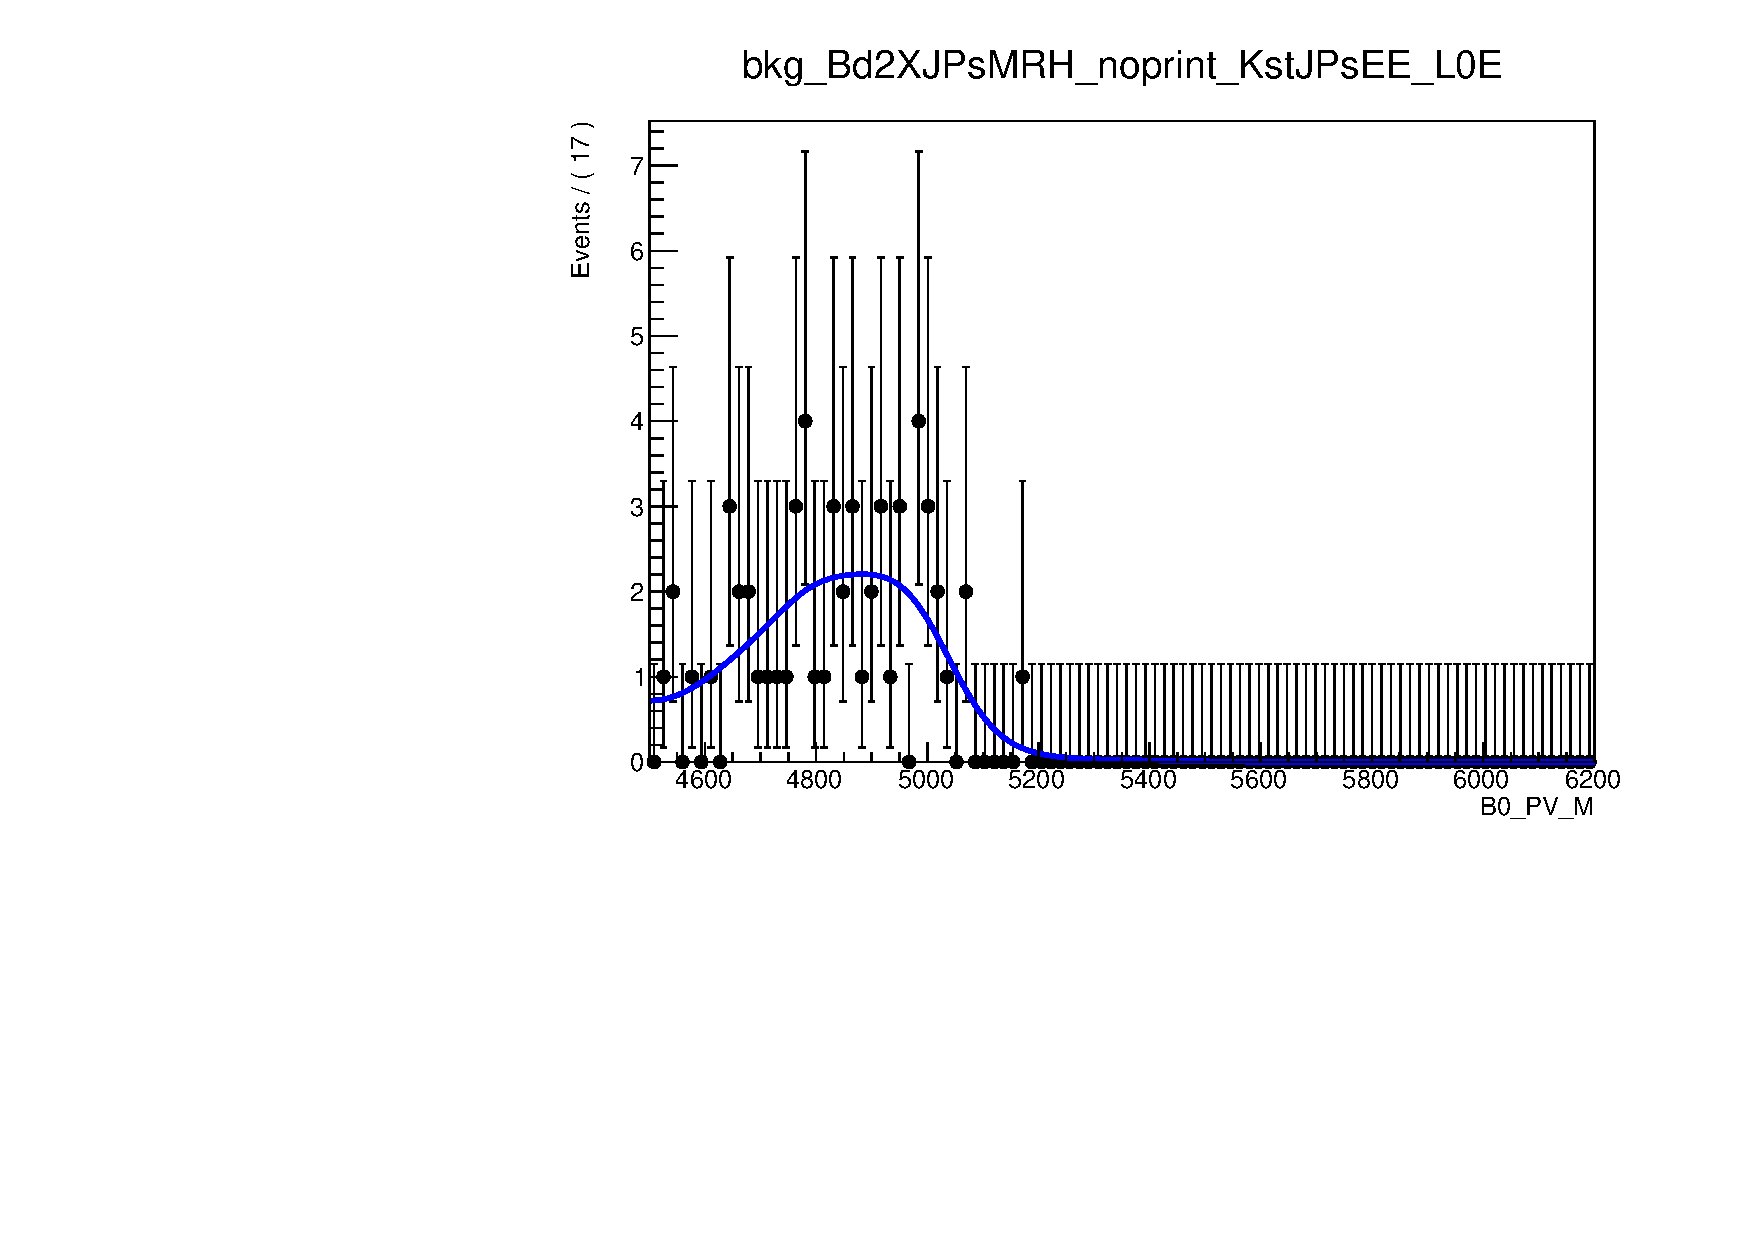
\includegraphics[width=0.49\textwidth]{RKst/figs/Fit/fit_EE/rooKeysModel_bkg_Bd2XJPsMRH_noprint_KstJPsEE_L0E.pdf}
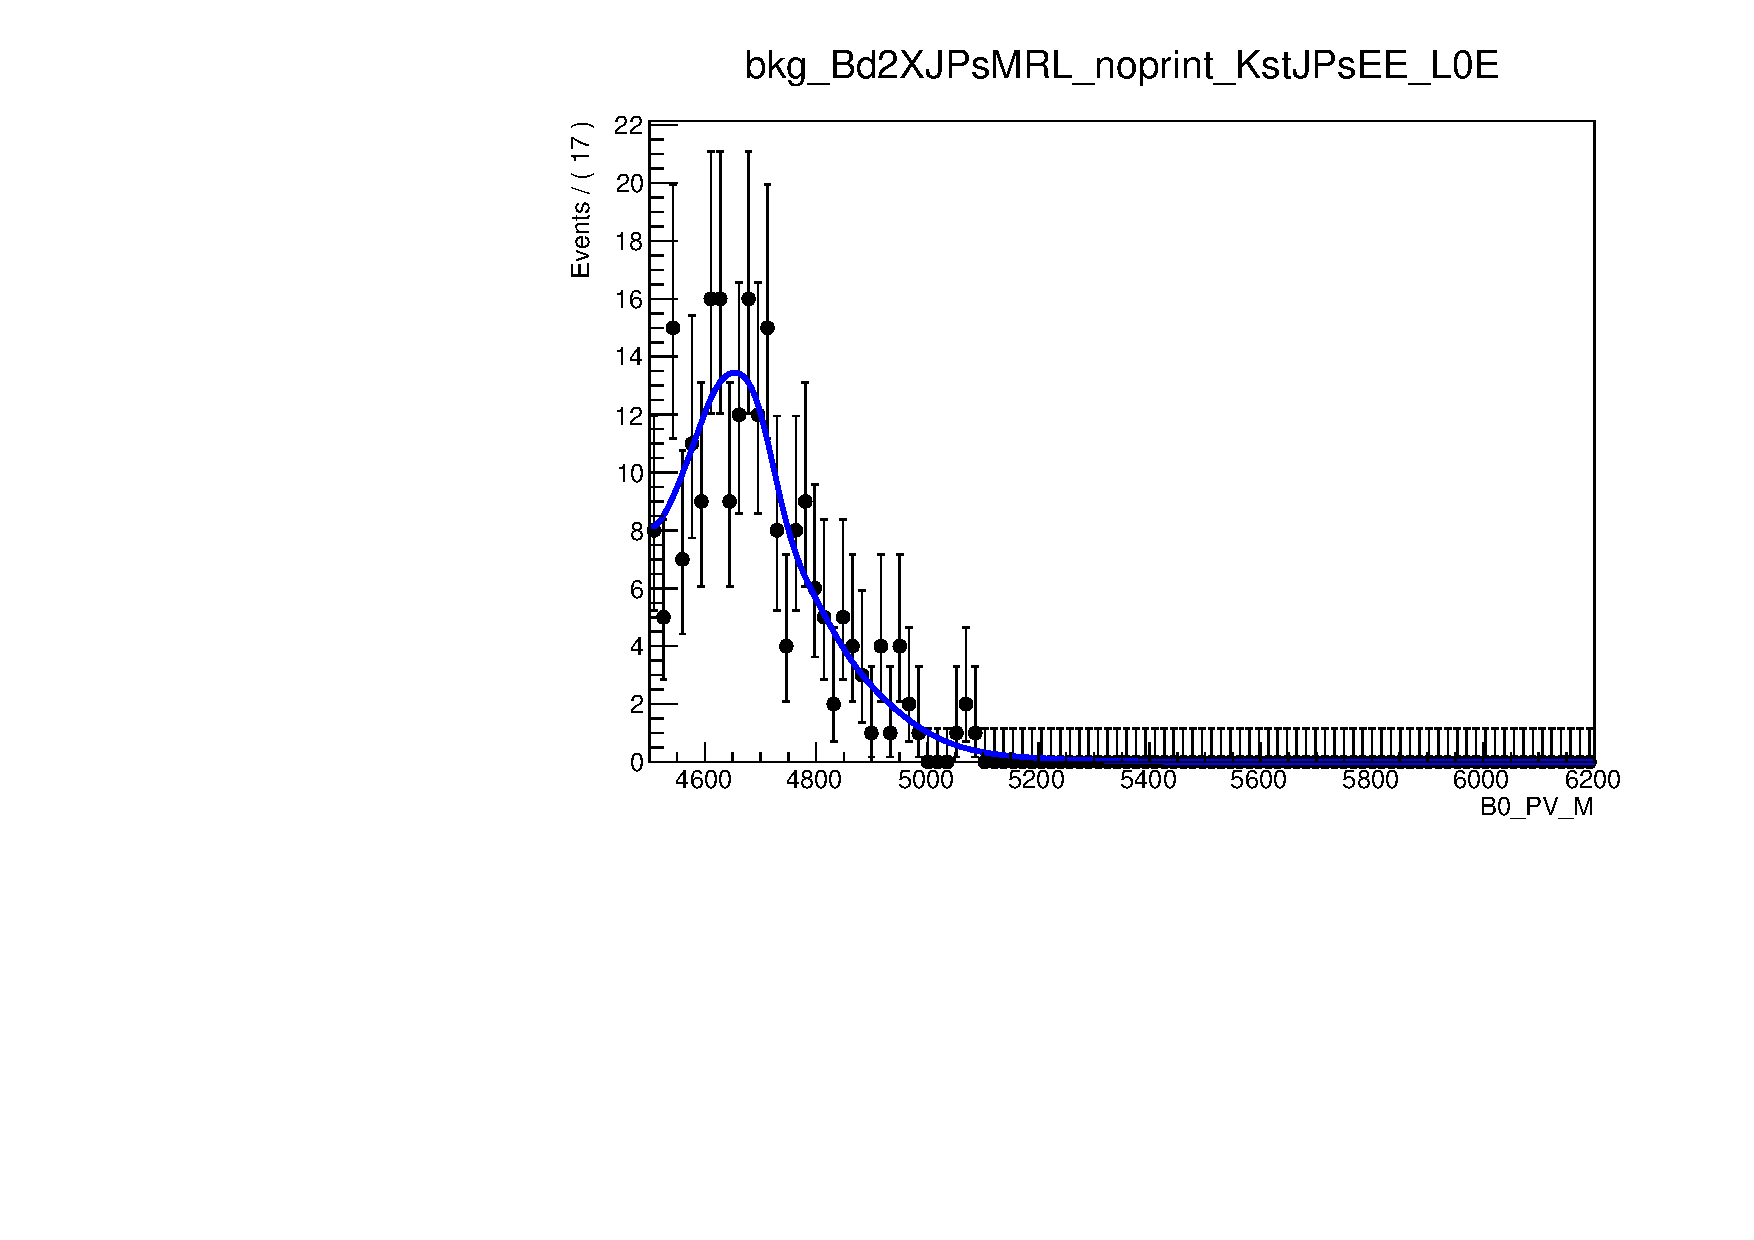
\includegraphics[width=0.49\textwidth]{RKst/figs/Fit/fit_EE/rooKeysModel_bkg_Bd2XJPsMRL_noprint_KstJPsEE_L0E.pdf}
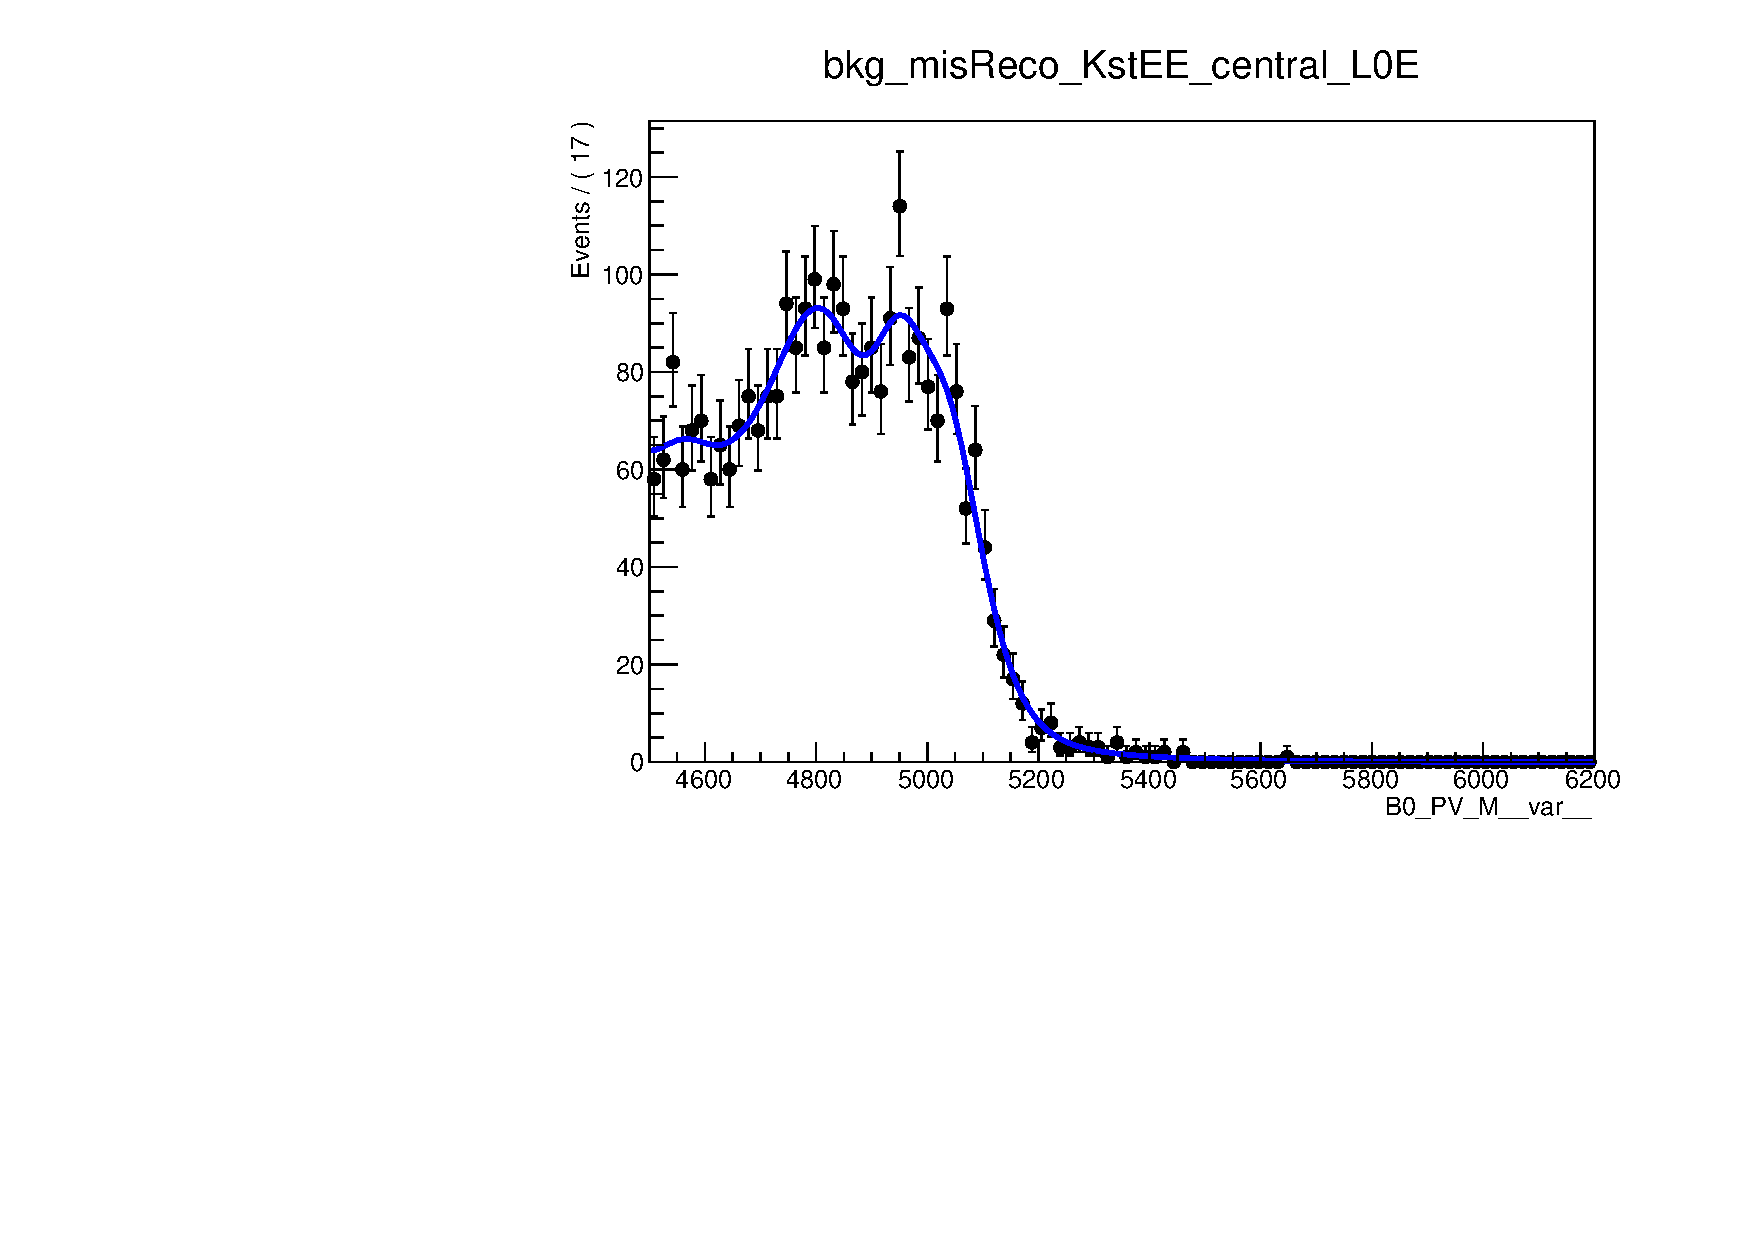
\includegraphics[width=0.49\textwidth]{RKst/figs/Fit/fit_EE/rooKeysModel_bkg_misReco_KstEE_central_L0E.pdf}
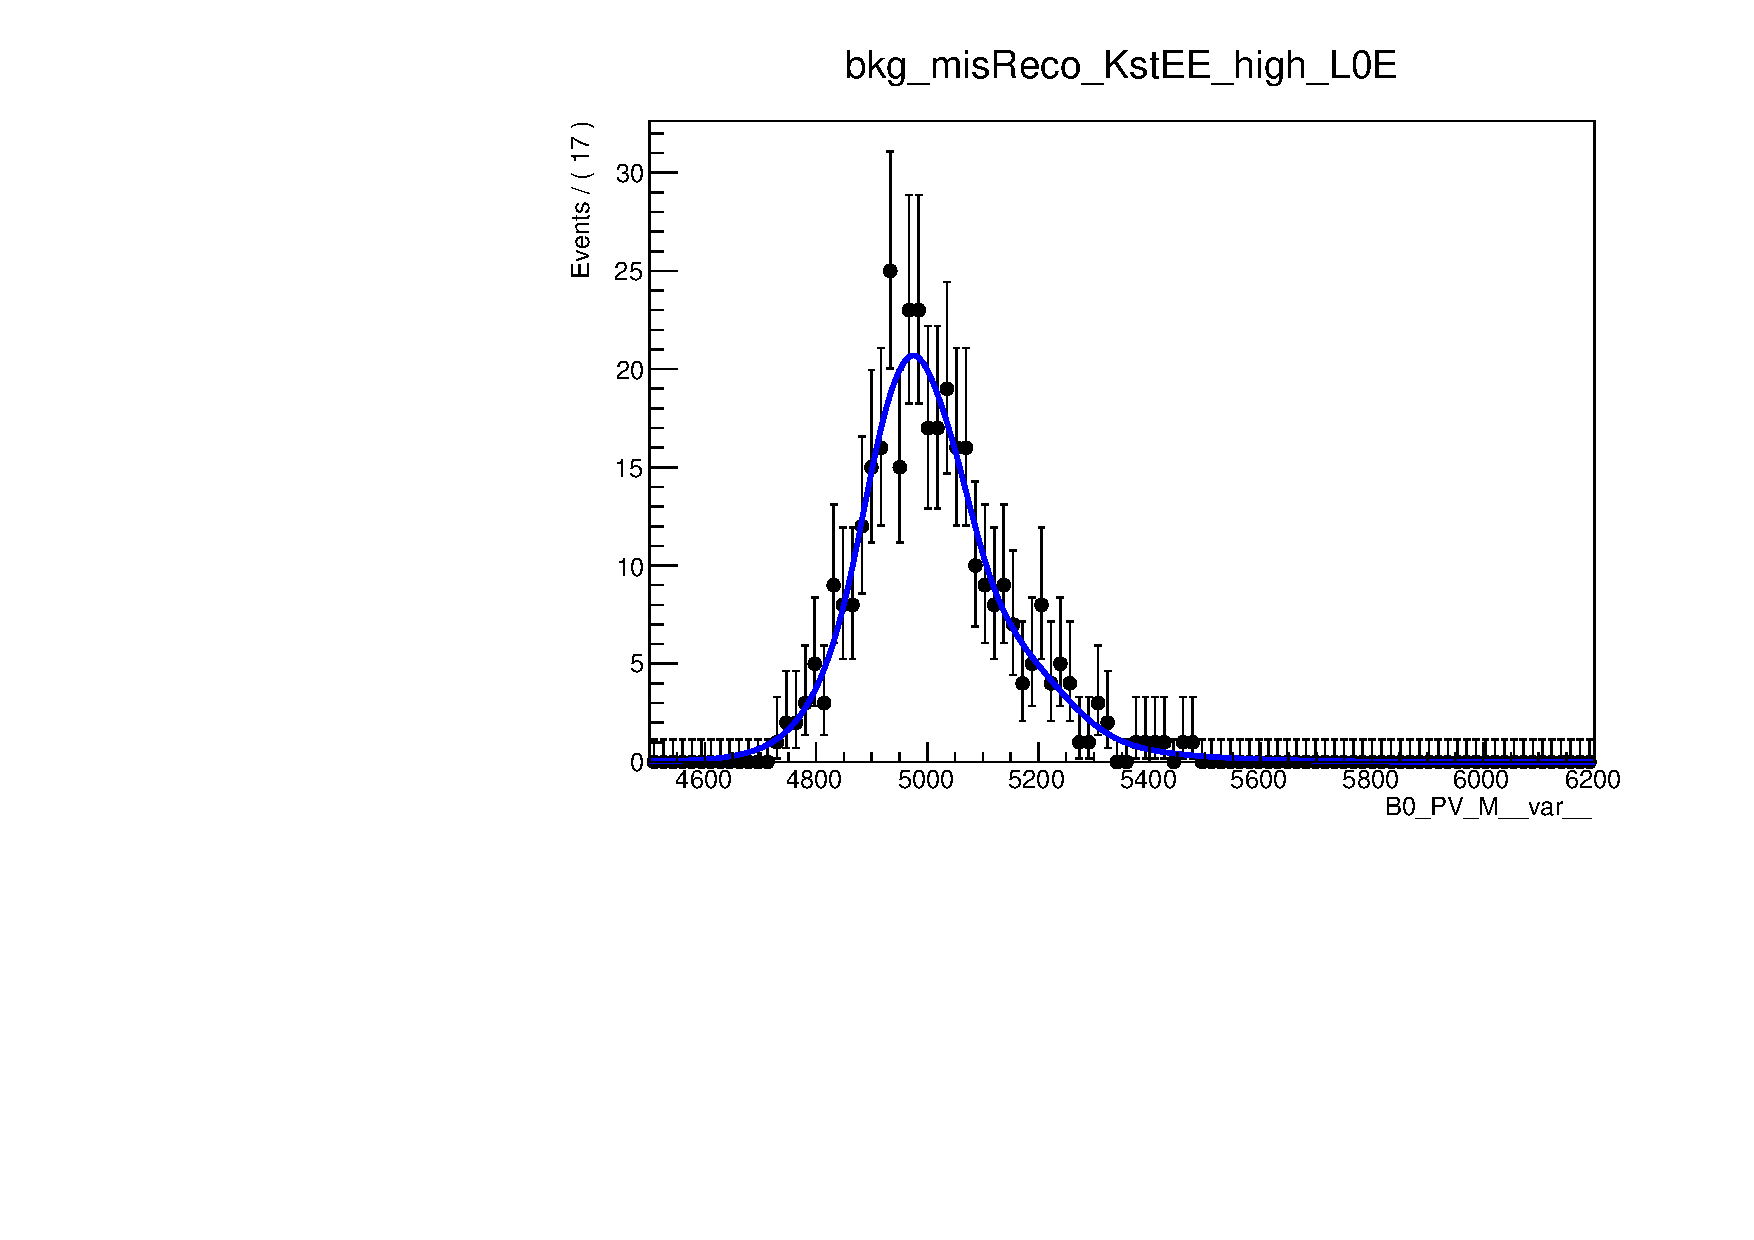
\includegraphics[width=0.49\textwidth]{RKst/figs/Fit/fit_EE/rooKeysModel_bkg_misReco_KstEE_high_L0E.pdf}
\caption{Distributions of the \mKpiee invariant mass for the (top left) hadronic and (top right) leptonic mis-reconstructed background to \BdToKstJPsee. Distributions of the \mKpiee invariant mass for decays involving
higher \Kstarz resonances in the (bottom left) central- and (bottom right) high-\qsq interval.}
\label{fig:misreco}
%\end{figure}

\vspace{1cm}

%\begin{figure}[t!]
\centering
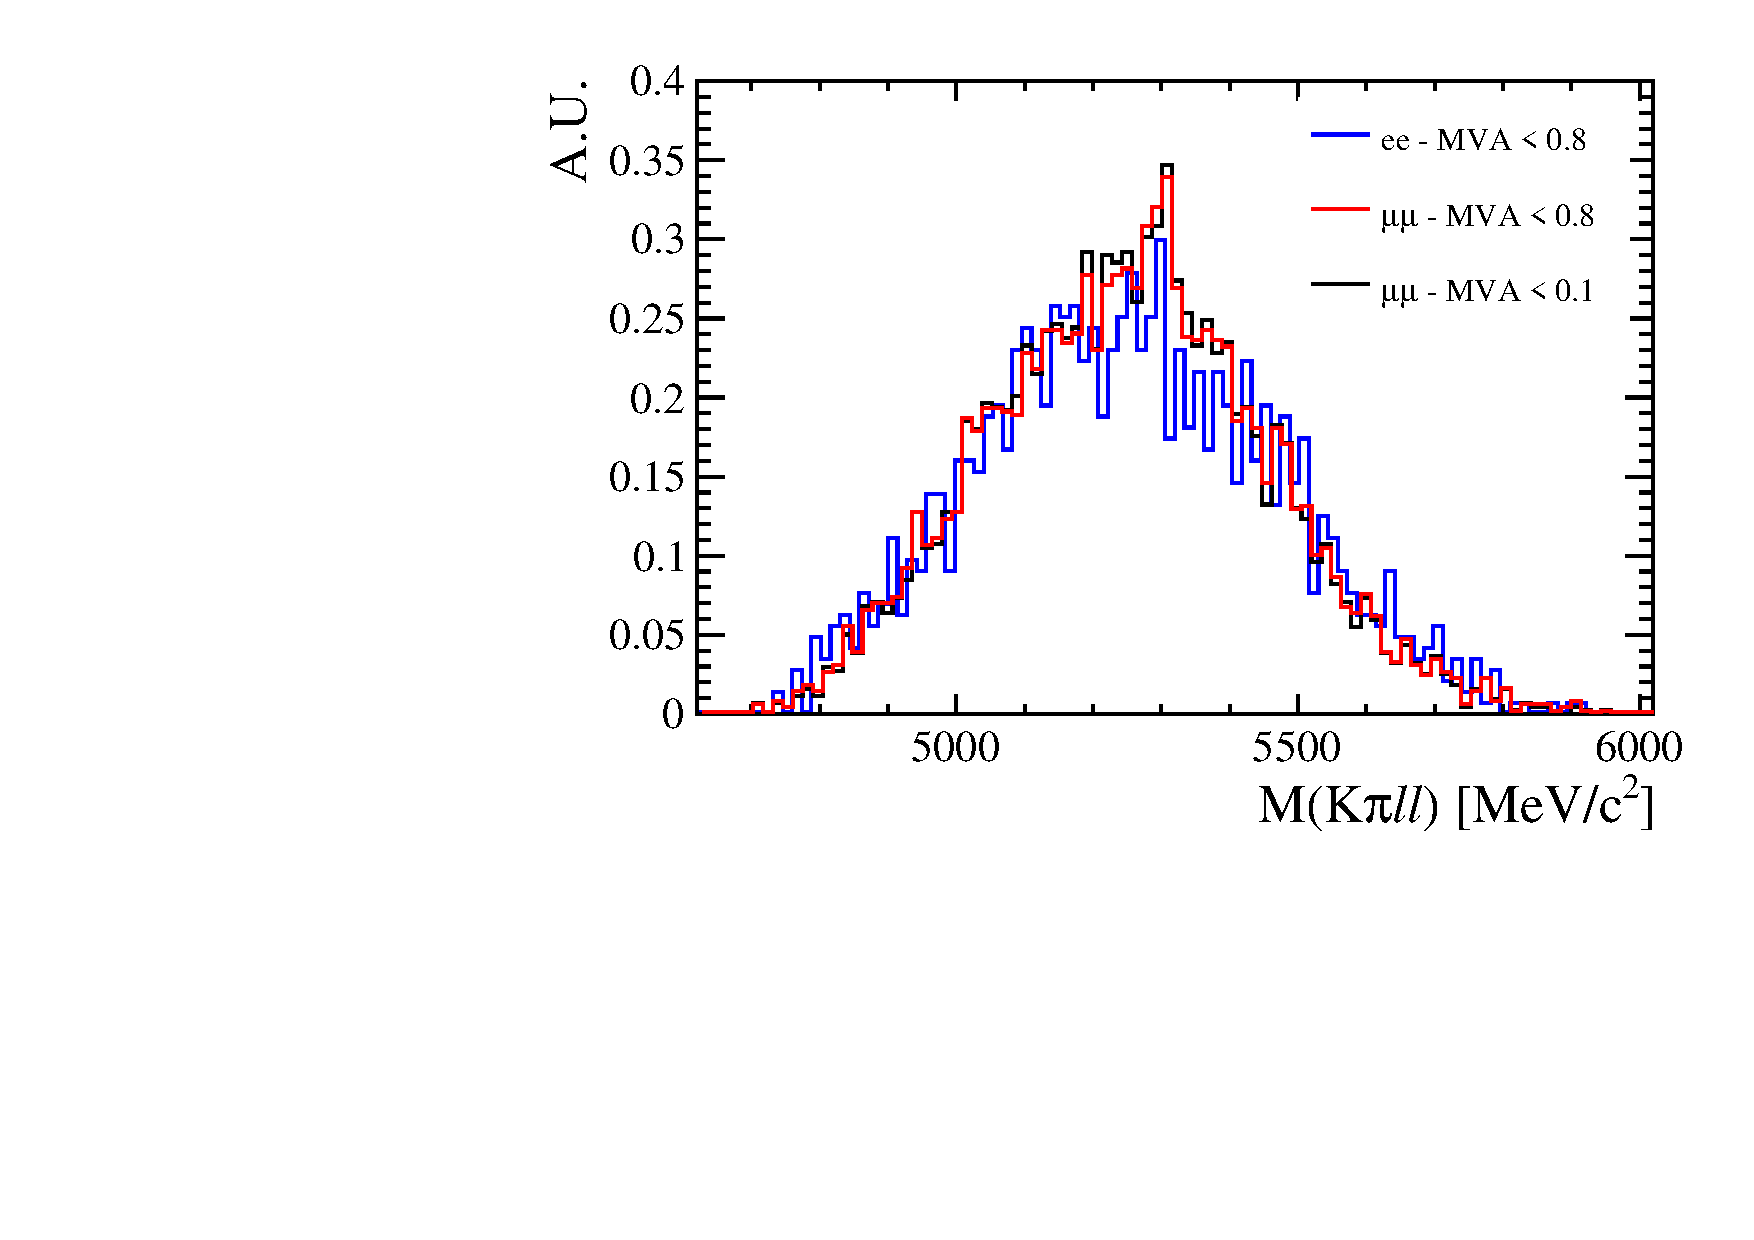
\includegraphics[width=0.6\textwidth]{RKst/figs/Background/highq2_comb.pdf}
\caption{Distributions of the \mKpill invariant mass for \BdToKstll candidates selected with a reversed cuts on the NN output.}
\label{fig:highq2_comb}
\end{figure}

\clearpage

\subsubsection{Summary of the fit to the electron samples}

In summary, the free parameters in the fit to data are:
%
\begin{itemize}
\item the \BdToKstJPsee, \BdToKstPsiee and \BdToKstGee yields in each trigger category;
\item the $r_{ee}$ ratio common to all trigger categories; one for the low, one for the central- and one for the high-\qsq region;
\item one mass shift, $m'$, and one width scale factor, $c$, for the signal PDF common between \BdToKstJPsee and \BdToKstee,
but different for the three trigger categories and for \BdToKstPsiee and \BdToKstGee;
\item the yield and slope, when applicable (e.g. no slope at high-\qsq), of the combinatorial background in each trigger category and for each channel;
\item the yield of the backgrounds when not fixed as described in the previous section.
\end{itemize}

Fits to simulated \BdToKstJPsee candidates are shown in Appendix~\ref{app:RKMCfits}, while
fits to real candidates are shown in Fig.~\ref{fig:fitJPsEE} for the normalisation channel, in Fig.~\ref{fig:fitsEE} 
for the rare channel and in Fig.~\ref{fig:fitsControlEE} for the control channels.
For simplicity the latter two figures show the sub of the three trigger categories, while the separate plots are
reported in Appendix~\ref{app:RKDatafits}, where fitted parameters are also reported on the plots.

In the high-\qsq interval, above 15~\gevgevcccc, the efficiency for the
L0Hadron trigger becomes very low as the \Kstar has very low momentum.
In this region only 9 candidates are found spread in the interval
$4500 < m(K\pi ee) < 6000$ \mevcc. Therefore
only L0E and L0I triggered events are fitted in this region.

\subsection{Event yields}

Table~\ref{tab:RKst_yields} reports raw yields obtained from the
fits described in the previous subsections. The values for the rare channels are not
directly floating in the fits but, as described in Sec.~\ref{sec:rkst_fits}, they are parameterised
as a function of the number of resonant events found and the ratios $R_{ee}$ and $R_{\mu\mu}$
between the resonant and rare branching fractions. Measured values of these ratios are reported 
in Tab.~\ref{tab:RKst_results}.

\begin{table}
\centering
\begin{tabular}{|c|c|c|c|}
\hline
 Sample 			& 1--6~\gevgevcccc 			& 15--20~\gevgevcccc 		& \jpsi  \\ \hline
$\mu\mu$ 		& $ 626.47  \pm 29.60  $ 		& $ 605.09  \pm 27.44 $ 		& $ 333112.99  \pm 603.77 $ \\
$ee$ L0E 			& $ 131.62   \pm  17.11$   	& $ 136.69  \pm 27.34 $ 		& $ 48601.38  \pm 326.48 $ \\
$ee$ L0H 			& $ 31.65   \pm  4.16$ 		& 			-- 			& $ 4323.62  \pm 94.49 $ \\
$ee$ L0I 			& $ 49.59   \pm  6.48$ 		& 			-- 			& $ 12791.37  \pm 172.47 $ \\
\hline
 \end{tabular}
\caption{Raw yields of events found fitting invariant mass distributions of the rare and resonant events. }
\label{tab:RKst_yields}
\end{table}


\begin{figure}[h!]
\centering
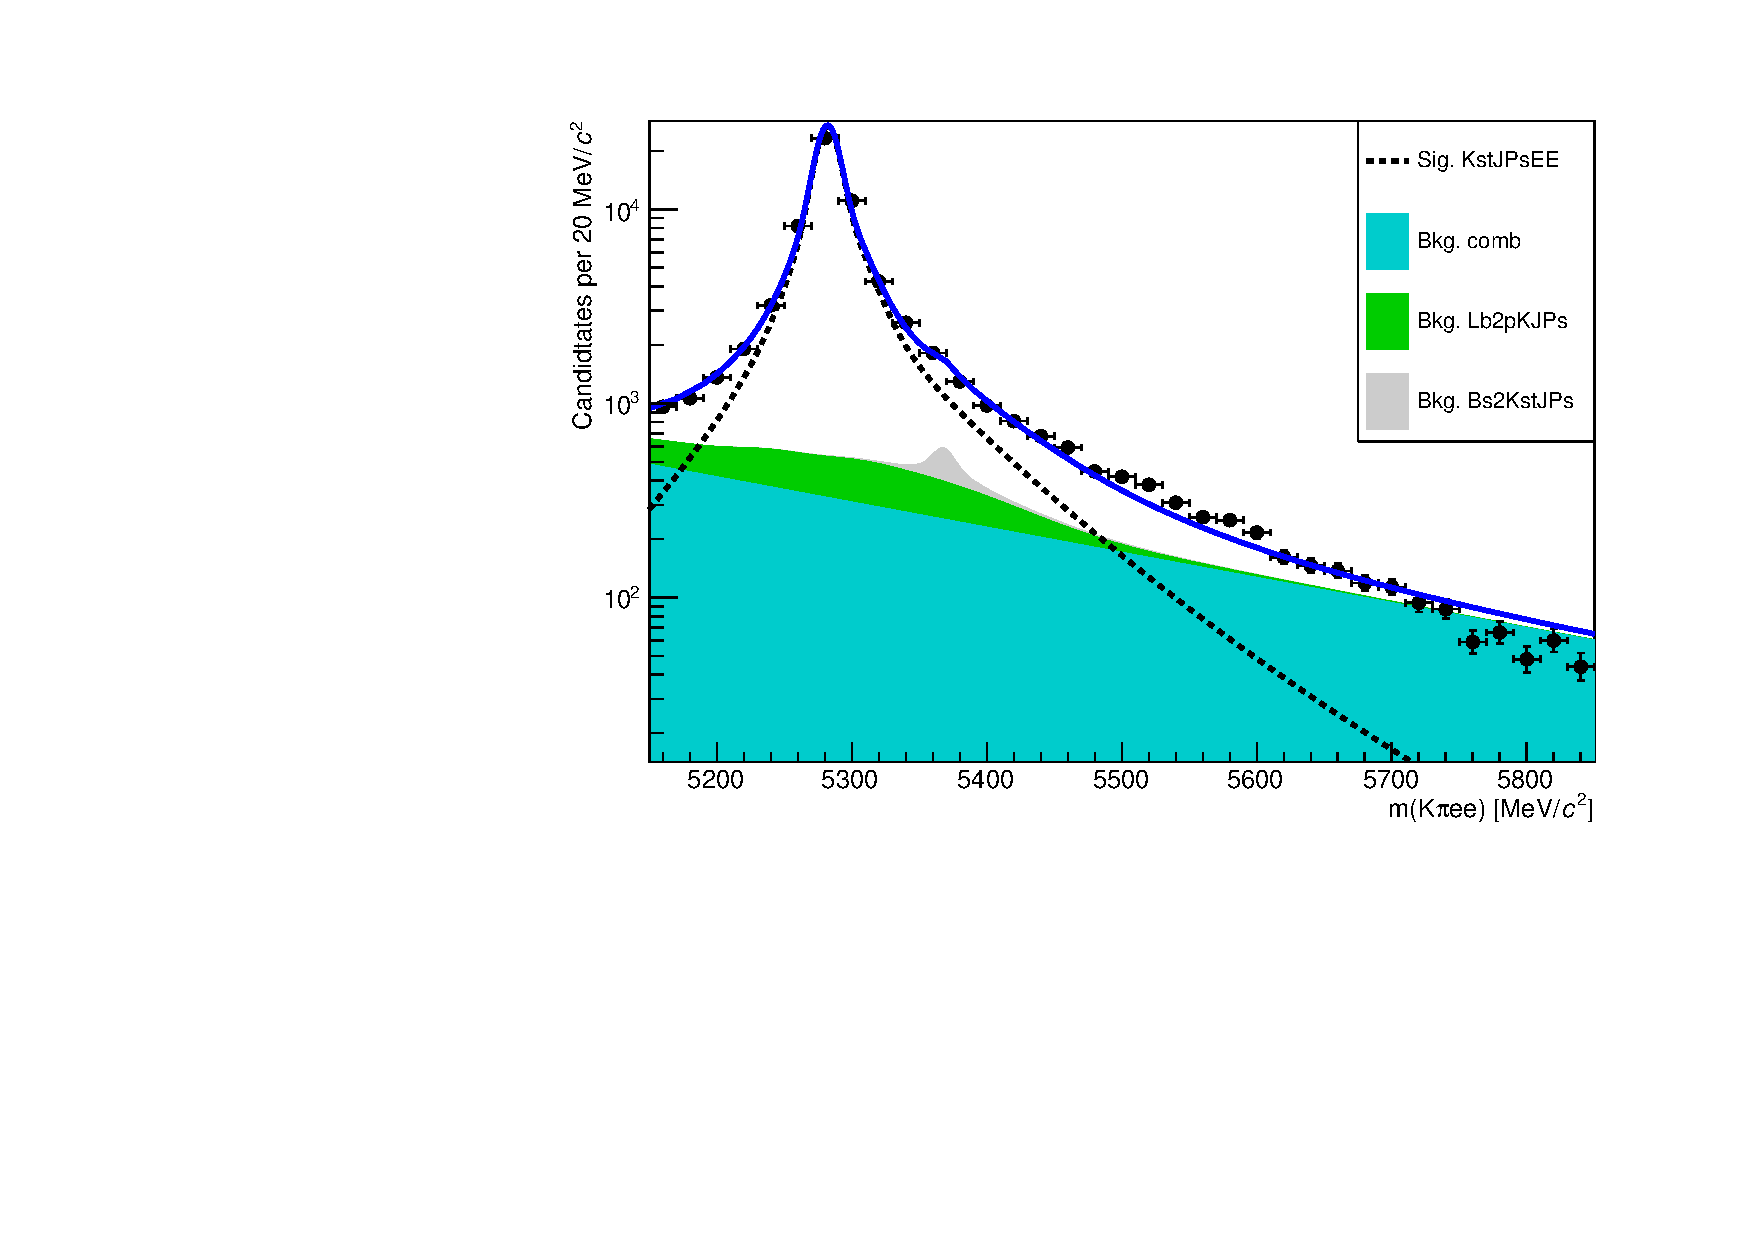
\includegraphics[width=0.6\textwidth]{RKst/figs/Fit/fit_EE/fit_JPs_L_log.pdf}
\caption{Fit to the mass constrained \mKpiee invariant mass of \BdToKstJPsee candidates.
The dashed black line (shaded shapes) represents the signal (background) PDF.}
\label{fig:fitJPsEE}
\end{figure}
%
\begin{figure}[h!]
\centering
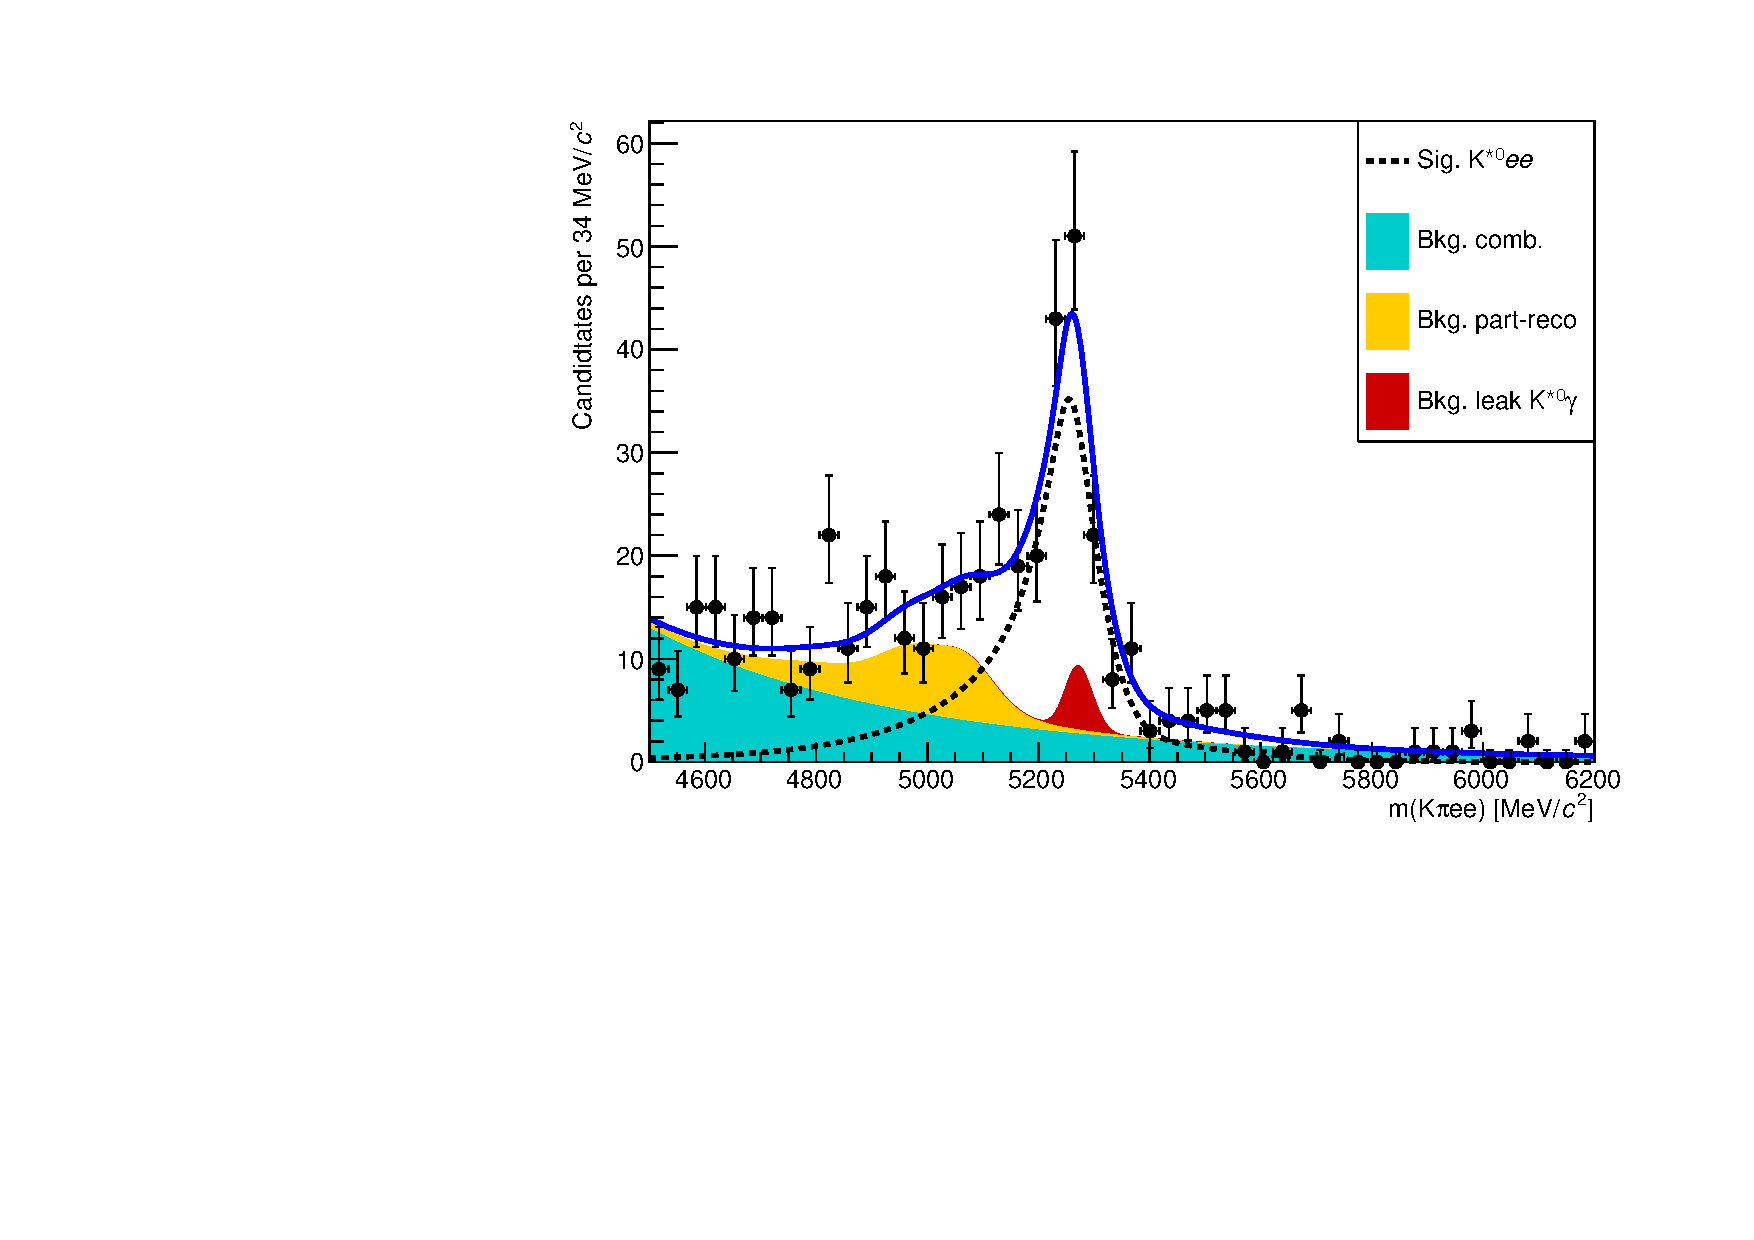
\includegraphics[width=0.6\textwidth]{RKst/figs/Fit/fit_EE/fit_EEl.pdf}
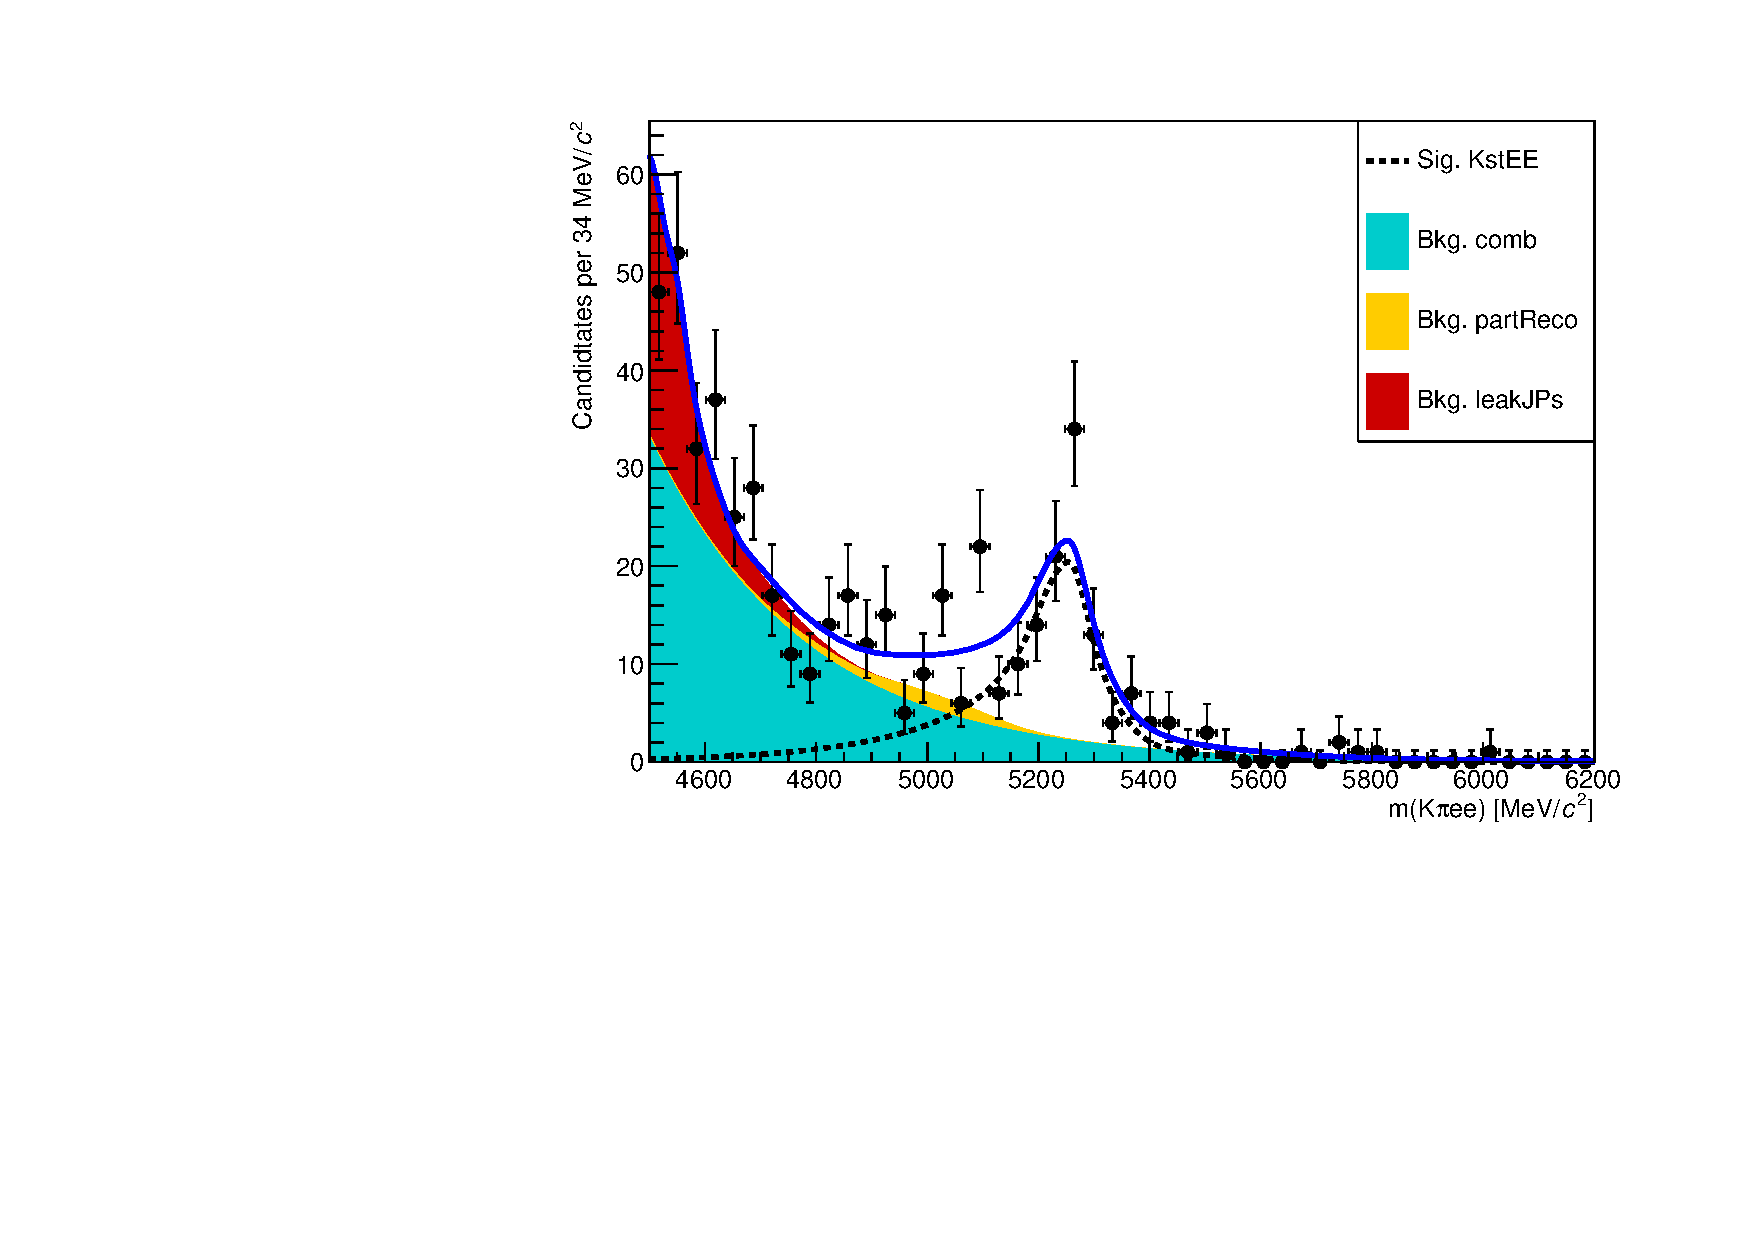
\includegraphics[width=0.6\textwidth]{RKst/figs/Fit/fit_EE/fit_EEc.pdf}
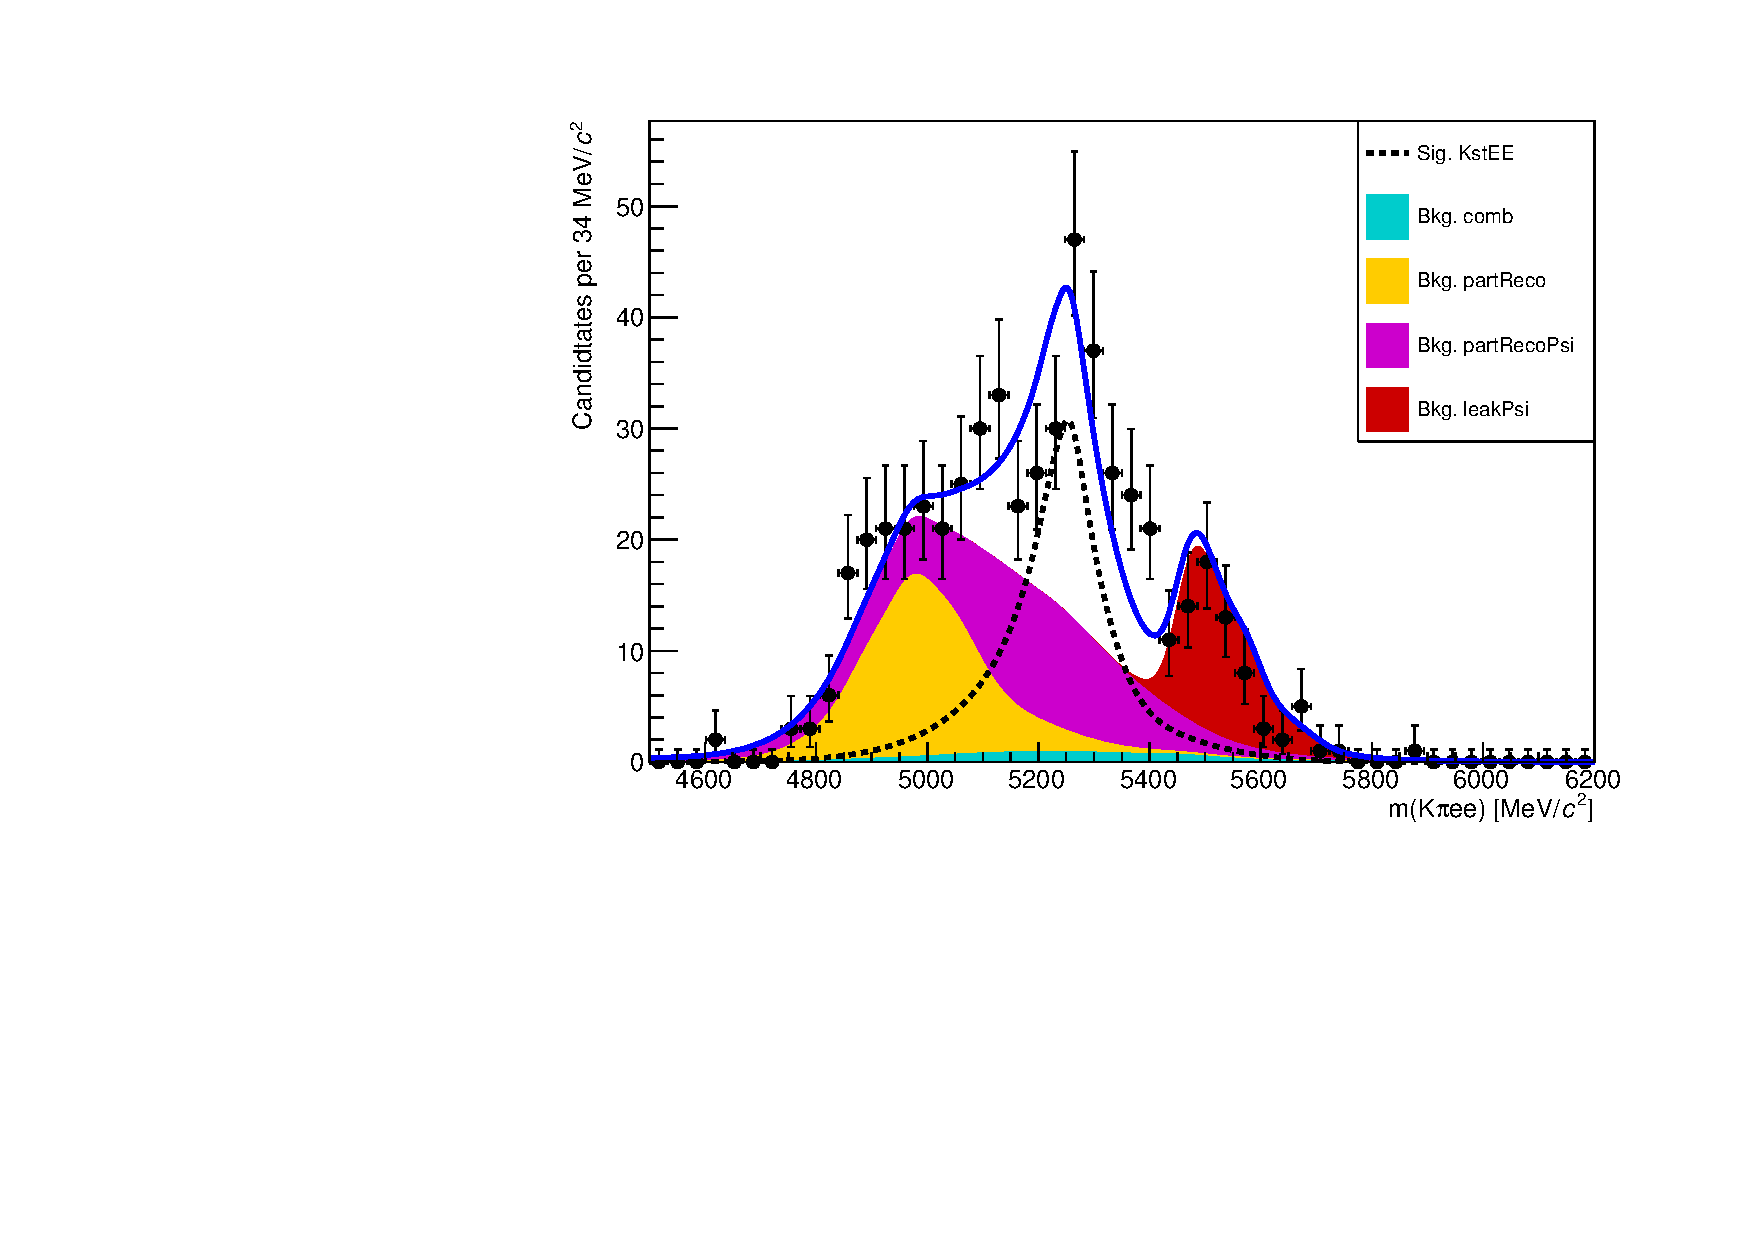
\includegraphics[width=0.6\textwidth]{RKst/figs/Fit/fit_EE/fit_EEh.pdf}
\caption{Fit to the \mKpiee invariant mass of \BdToKstee candidates. From top to bottom for the low-, central-
and high-\qsq intervals. The dashed black line (shaded shapes) represents the signal (background) PDF.}
\label{fig:fitsEE}
\end{figure}
%
\begin{figure}[h!]
\centering
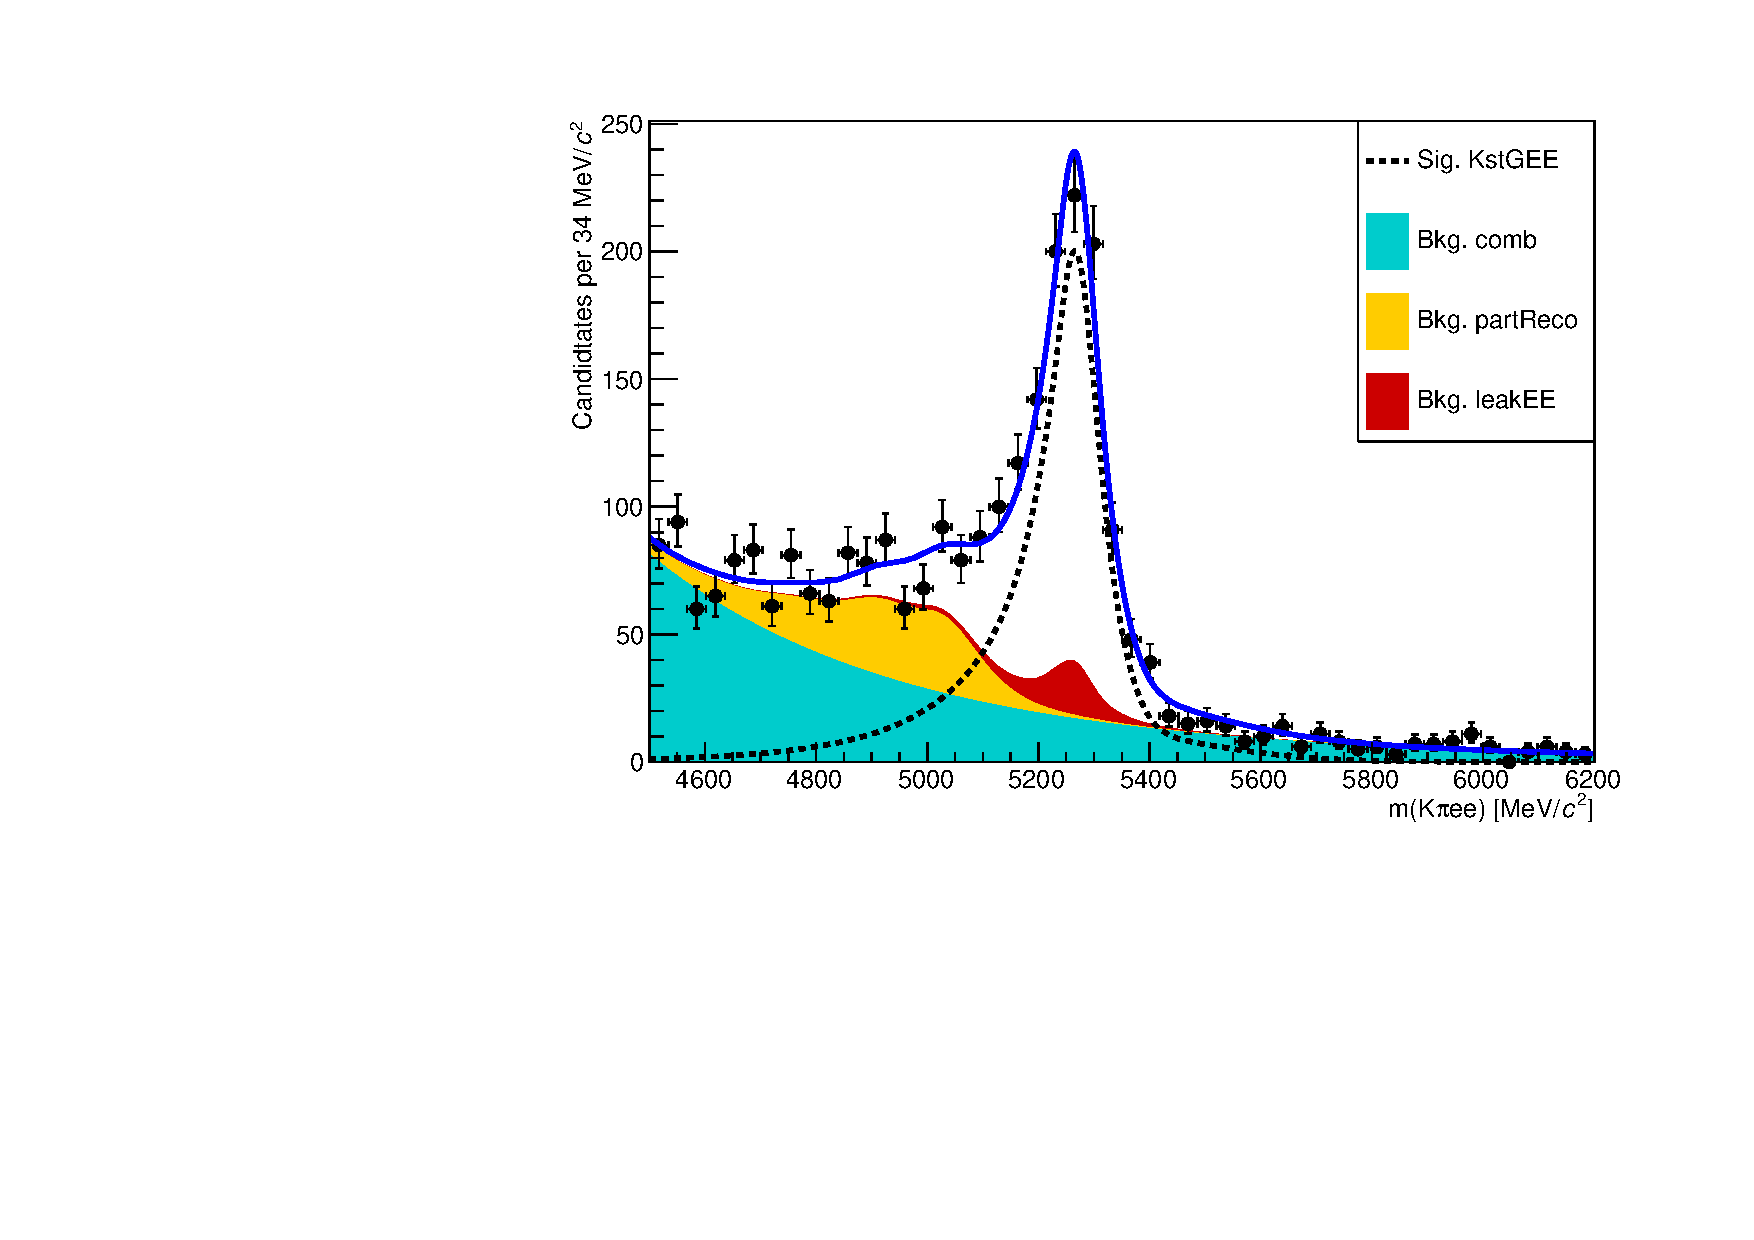
\includegraphics[width=0.6\textwidth]{RKst/figs/Fit/fit_EE/fit_G.pdf}
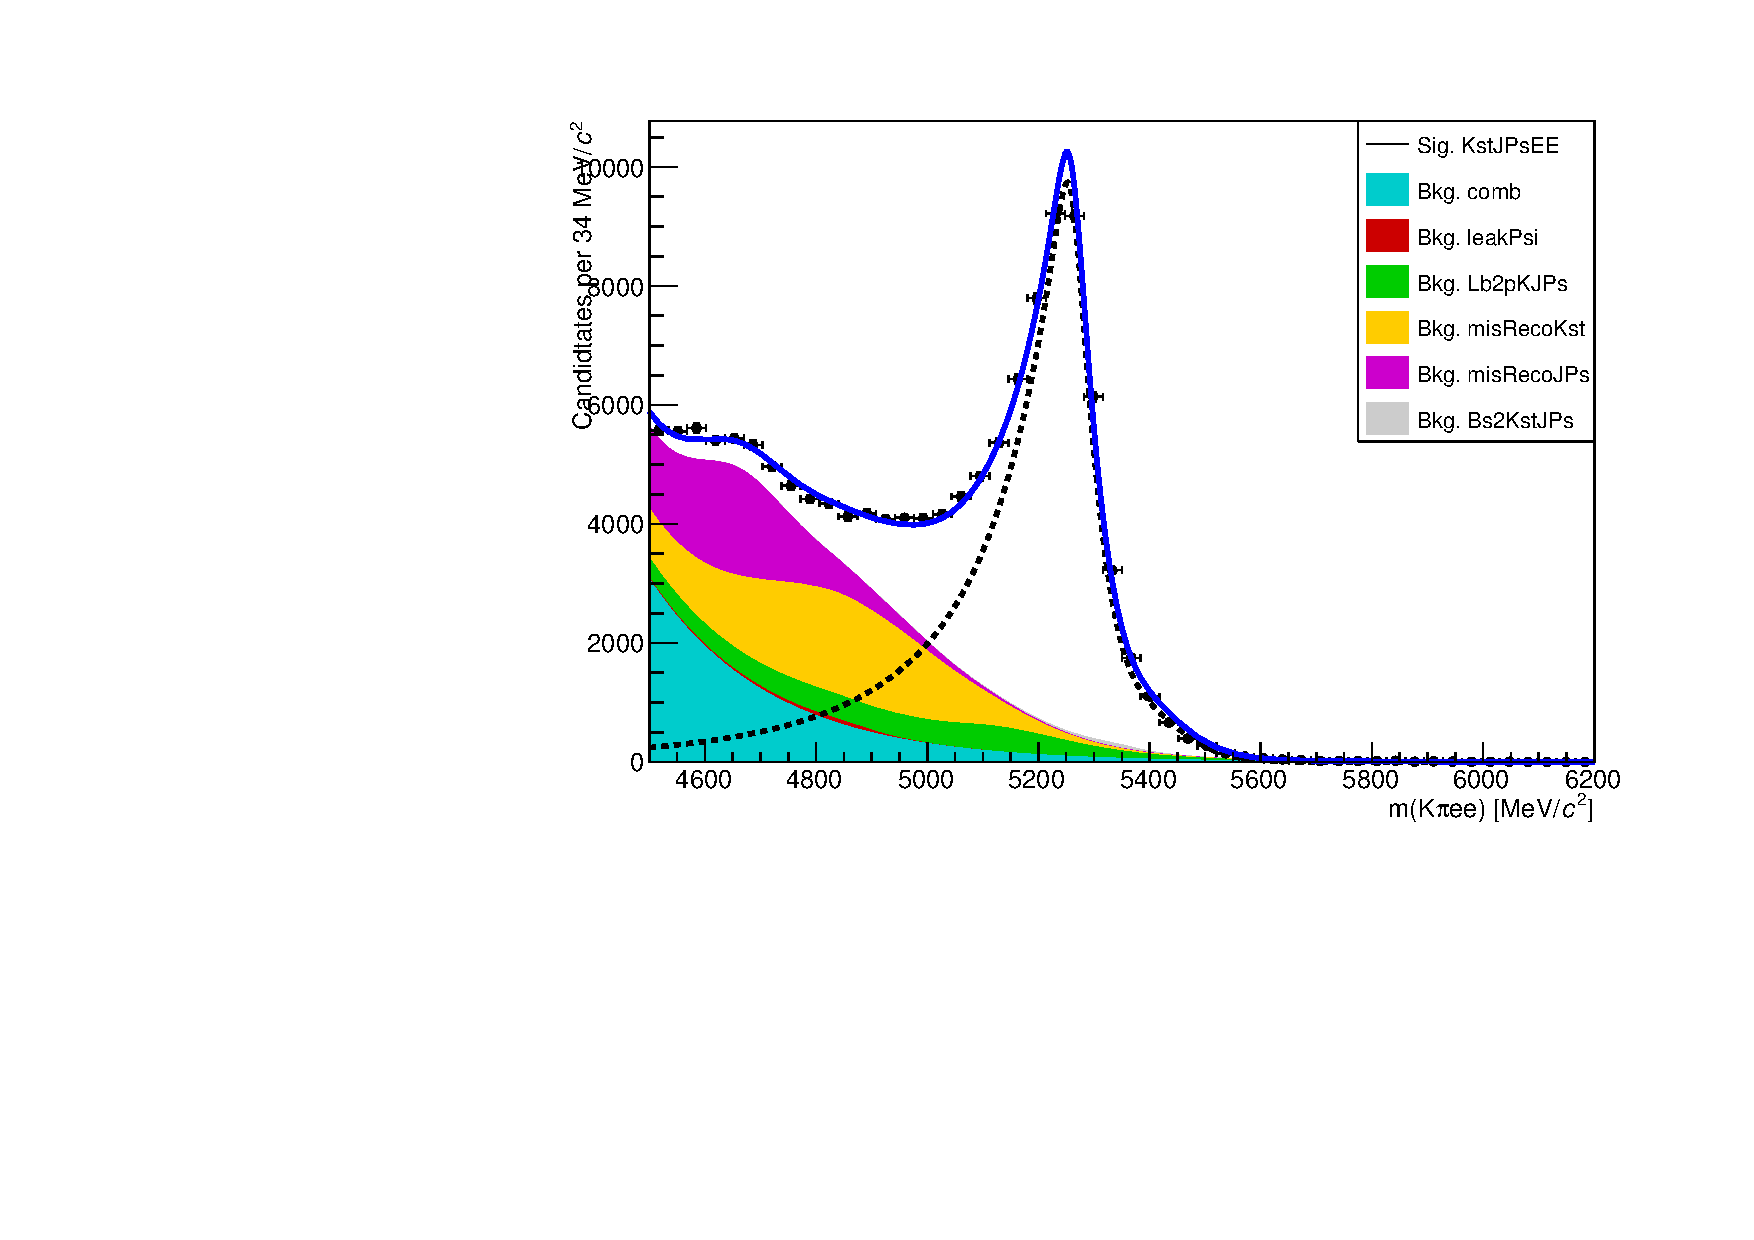
\includegraphics[width=0.6\textwidth]{RKst/figs/Fit/fit_EE/fit_JPs.pdf}
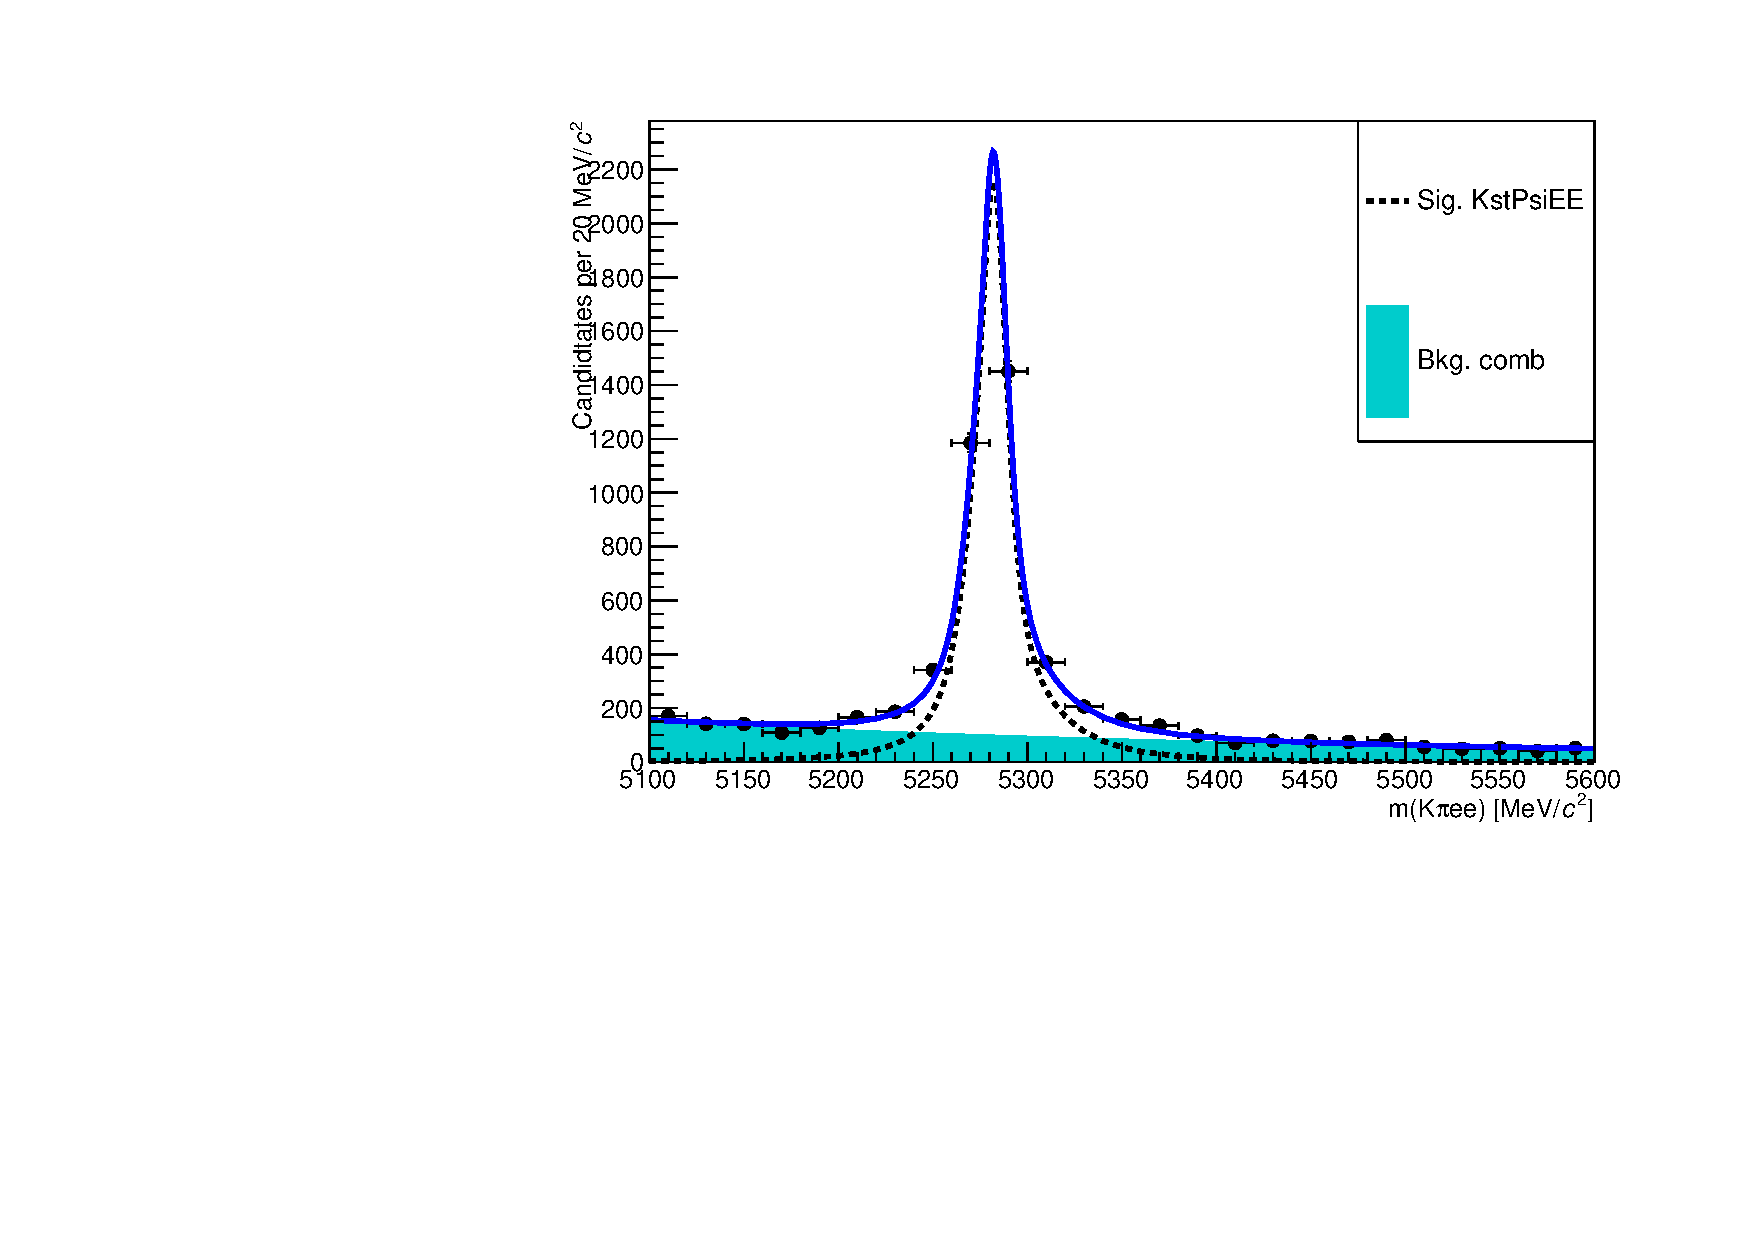
\includegraphics[width=0.6\textwidth]{RKst/figs/Fit/fit_EE/fit_Psi.pdf}
\caption{Fit to the \mKpiee invariant mass of control channel candidates.
From top to bottom: invariant mass distribution without mass constraint of \BdToKstGee
and \BdToKstJPsee candidates and mass constrained mass of \BdToKstPsiee candidates.
The dashed black line (shaded shapes) represents the signal (background) PDF.}
\label{fig:fitsControlEE}
\end{figure}

\clearpage

